\subsection{Теоретический минимум к кр 1}


\begin{enumerate}
	\item Классическое определение вероятности
	\item Определение условной вероятности
	\item Определение независимости случайных событий
	\item Формула полной вероятности
	\item Формула Байеса
	\item Функция распределения случайной величины. Определение и свойства.
	\item Функция плотности. Определение и свойства.
	\item Математическое ожидание. Определения для дискретного и абсолютно непрерывного случаев. Свойства.
	\item Дисперсия. Определение и свойства.
	\item Законы распределений. Определение, $\E(X)$, $\Var(X)$:
	\begin{enumerate}
	\item Биномиальное распределение
	\item Распределение Пуассона
	\item Геометрическое распределение
	\item Равномерное распределение
	\item Экспоненциальное распределение
	\end{enumerate}
\end{enumerate}


\subsection{Задачный минимум к кр 1}

\begin{enumerate}
\item  Пусть $\P(A) = 0.3, \P(B) = 0.4, \P(A\cap B) = 0.1 $. Найдите
	\begin{enumerate}
		\item  $\P(A|B)$
		\item  $\P(A\cup B)$
		\item  Являются ли события $A$ и $B$ независимыми?
	\end{enumerate}



\item  Пусть $\P(A) = 0.5, \P(B) = 0.5, \P(A\cap B) = 0.25 $. Найдите
\begin{enumerate}
	\item  $\P(A|B)$
	\item  $\P(A\cup B)$
	\item  Являются ли события $A$ и $B$ независимыми?
\end{enumerate}



\item  Карлсон выложил кубиками слово КОМБИНАТОРИКА. Малыш выбирает наугад четыре кубика и выкладывает их в случайном порядке.
Найдите вероятность того, что при этом получится слово КОРТ.


\item  Карлсон выложил кубиками слово КОМБИНАТОРИКА. Малыш выбирает наугад четыре кубика и выкладывает их в случайном порядке.
Найдите вероятность того, что при этом получится слово РОТА.

\item  В первой урне 7 белых и 3 черных шара, во второй урне 8 белых и 4 черных
шара, в третьей урне 2 белых и 13 черных шаров. Из этих урн наугад выбирается одна урна. Какова вероятность того, что шар, взятый наугад из выбранной урны, окажется белым?


\item  В первой урне 7 белых и 3 черных шара, во второй урне 8 белых и 4 черных
шара, в третьей урне 2 белых и 13 черных шаров. Из этих урн наугад выбирается одна урна. Какова вероятность того, что была выбрана первая урна, если шар, взятый наугад из выбранной урны, оказался белым?


\item  В операционном отделе банка работает 80\% опытных сотрудников и 20\%
неопытных. Вероятность совершения ошибки при очередной банковской операции
опытным сотрудником равна 0.01, а неопытным — 0.1. Найдите вероятность совершения ошибки при очередной банковской операции в этом отделе.


\item  В операционном отделе банка работает 80\% опытных сотрудников и 20\%
неопытных. Вероятность совершения ошибки при очередной банковской операции
опытным сотрудником равна 0.01, а неопытным — 0.1. Известно, что при очередной банковской операции была допущена ошибка. Найдите вероятность того, что ошибку допустил неопытный сотрудник.

\item  Пусть случайная величина $X$ имеет таблицу распределения:

\begin{tabular}{ ll l l}
	\toprule
	$X$ & -1  & 0  & 1 \\
	$\P_X$ & 0.25  & c  & 0.25 \\
  \bottomrule
\end{tabular}

Найдите
	\begin{enumerate}
	\item константу $c$
	\item $\P(\{X \geq 0\})$
	\item $\P(\{X < -3\}])$
	\item $\P(\{X \in [-\frac{1}{2}; \frac{1}{2}]\})$
	\item функцию распределения случайной величины $X$
	\item имеет ли случайная величина $X$ плотность распределения?
	\end{enumerate}


\item  Пусть случайная величина $X$ имеет таблицу распределения:

\begin{tabular}{ llll}
\toprule
$X$ & -1  & 0  & 1 \\
$\P_X$ & 0.25  & c  & 0.25 \\
\bottomrule
\end{tabular}

Найдите
\begin{enumerate}
	\item константу $c$
	\item $\E(X)$
	\item $\E(X^2)$
	\item $\Var(X)$
	\item $\E(|X|)$
\end{enumerate}

\item  Пусть случайная величина $X$ имеет таблицу распределения:

\begin{tabular}{ lll l}
\toprule
$X$ & -1  & 0  & 1 \\
$\P_X$ & 0.25  & c  & 0.5 \\
\bottomrule
\end{tabular}

Найдите
	\begin{enumerate}
	\item константу $c$
	\item $\P(\{X \geq 0\})$
	\item $\P(\{X < -3\}])$
	\item $\P(\{X \in [-\frac{1}{2}; \frac{1}{2}]\})$
	\item функцию распределения случайной величины $X$
	\item имеет ли случайная величина $X$ плотность распределения?
\end{enumerate}

\item  Пусть случайная величина $X$ имеет таблицу распределения:

\begin{tabular}{ l l l l}
  \toprule
$X$ & -1  & 0  & 1 \\
$\P_X$ & 0.25  & c  & 0.5 \\
\bottomrule
\end{tabular}

Найдите
\begin{enumerate}
	\item константу $c$
	\item $\E(X)$
	\item $\E(X^2)$
	\item $\Var(X)$
	\item $\E(|X|)$
\end{enumerate}

\item Пусть случайная величина $X$ имеет биномиальное распределение с
параметрами $n = 4$ и $\P = \frac{3}{4}$.
 Найдите
\begin{enumerate}
	\item $\P(\{X = 0\})$
	\item $\P(\{X > 0\})$
	\item $\P(\{X < 0\})$
	\item $\E(X)$
	\item $\Var(X)$
	\item  наиболее вероятное значение, которое принимает случайная величина $X$
\end{enumerate}

\item Пусть случайная величина $X$ имеет биномиальное распределение с
параметрами $n = 5$ и $\P = \frac{2}{5}$.
Найдите
\begin{enumerate}
	\item $\P(\{X = 0\})$
	\item $\P(\{X > 0\})$
	\item $\P(\{X < 0\})$
	\item $\E(X)$
	\item $\Var(X)$
	\item  наиболее вероятное значение, которое принимает случайная величина $X$
\end{enumerate}


\item  Пусть случайная величина X имеет распределение Пуассона с параметром $\lambda = 100$ . Найдите
\begin{enumerate}
	\item $\P(\{X = 0\})$
	\item $\P(\{X > 0\})$
	\item $\P(\{X < 0\})$
	\item $\E(X)$
	\item $\Var(X)$
	\item  наиболее вероятное значение, которое принимает случайная величина $X$
\end{enumerate}


\item  Пусть случайная величина X имеет распределение Пуассона с параметром $\lambda = 101$ . Найдите
\begin{enumerate}
	\item $\P(\{X = 0\})$
	\item $\P(\{X > 0\})$
	\item $\P(\{X < 0\})$
	\item $\E(X)$
	\item $\Var(X)$
	\item  наиболее вероятное значение, которое принимает случайная величина $X$
\end{enumerate}


\item В лифт 10-этажного дома на первом этаже вошли 5 человек. Вычислите
вероятность того, что на 6-м этаже выйдет хотя бы один человек.


\item В лифт 10-этажного дома на первом этаже вошли 5 человек. Вычислите
вероятность того, что на 6-м этаже не выйдет ни один человек.


\item При работе некоторого устройства время от времени возникают сбои.
Количество сбоев за сутки имеет распределение Пуассона. Среднее количество сбоев за сутки равно 3. Найти вероятность того, что в течение суток произойдет хотя бы один сбой.


\item При работе некоторого устройства время от времени возникают сбои.
Количество сбоев за сутки имеет распределение Пуассона. Среднее количество сбоев за сутки равно 3. Найти вероятность того, что за двое суток не произойдет ни одного сбоя.


\item Пусть случайная величина $X$ имеет плотность распределения

\[
f_X(x) =
	\begin{cases}
	c,\text{ при }  x \in [-1; 1] \\
	0,\text{ при } x \notin  [-1; 1] \\
	\end{cases}
\]

Найдите
\begin{enumerate}
	\item константу $c$
	\item $\P(\{X \leq 0\})$
	\item $\P(\{X \in [\frac{1}{2}; \frac{3}{2}]\})$
	\item $\P(\{X \in [2;3]\}$
	\item $F_X(x)$
\end{enumerate}


\item Пусть случайная величина $X$ имеет плотность распределения

\[
f_X(x) =
	\begin{cases}
	c,\text{ при }  x \in [-1; 1] \\
	0,\text{ при } x \notin  [-1; 1] \\
	\end{cases}
\]

Найдите
\begin{enumerate}
	\item константу $c$
	\item $\E(X)$
	\item $\E(X^2)$
	\item $\Var(X)$
	\item $\E(|X|)$
\end{enumerate}


\item Пусть случайная величина $X$ имеет плотность распределения

\[
f_X(x) =
	\begin{cases}
	cx,\text{ при }  x \in [0; 1] \\
	0,\text{ при } x \notin  [0; 1] \\
	\end{cases}
\]

Найдите
\begin{enumerate}
	\item константу $c$
	\item $\P(\{X \leq \frac{1}{2}\})$
	\item $\P(\{X \in [\frac{1}{2}; \frac{3}{2}]\})$
	\item $\P(\{X \in [2;3]\}$
	\item $F_X(x)$
\end{enumerate}


\item Пусть случайная величина $X$ имеет плотность распределения

\[
f_X(x) =
	\begin{cases}
	cx,\text{ при }  x \in [0; 1] \\
	0,\text{ при } x \notin  [0; 1] \\
	\end{cases}
\]

Найдите
\begin{enumerate}
	\item константу $c$
	\item $\E(X)$
	\item $\E(X^2)$
	\item $\Var(X)$
	\item $\E(\sqrt{X})$
\end{enumerate}
\end{enumerate}



\subsubsection*{Ответы}

\begin{enumerate}
	\item
			\begin{enumerate}
				\item 0.25
				\item 0.6
				\item нет
			\end{enumerate}
	\item
			\begin{enumerate}
				\item 0.5
				\item  0.75
				\item нет
			\end{enumerate}
	\item $\frac{4}{10 \cdot 11 \cdot 12 \cdot 13}$
	\item $\frac{4}{10 \cdot 11 \cdot 12 \cdot 13}$
	\item 0.5


	\item 0.42
	\item 0.028
	\item $\frac{5}{7}$
	\item
			\begin{enumerate}
				\item 0.5
				\item 0.75
				\item 0
				\item 0.5
			\end{enumerate}
	\item
			\begin{enumerate}
				\item 0.5
				\item  0
				\item  0.5
				\item  0.5
				\item  0.5
			\end{enumerate}
	\item
			\begin{enumerate}
				\item 0.25
				\item 0.75
				\item 0
				\item 0.5
			\end{enumerate}
	\item
			\begin{enumerate}
				\item 0.25
				\item 0.25
				\item 0.75
				\item 0.5
				\item 0.75
			\end{enumerate}
	\item
			\begin{enumerate}
				\item $\left( \frac{1}{4} \right) ^4$
				\item $1 - \left( \frac{1}{4} \right) ^4$
				\item 0
				\item 3
				\item 0.75
				\item 2, 3
			\end{enumerate}
	\item
			\begin{enumerate}
				\item $\left( \frac{3}{5} \right) ^5$
				\item $1 - \left( \frac{3}{5} \right) ^5$
				\item 0
				\item 2
				\item 1.2
				\item 2
			\end{enumerate}
	\item
			\begin{enumerate}
				\item $e^{-100}$
				\item $1 - e^{-100}$
				\item 0
				\item 100
				\item 100
			\end{enumerate}
	\item
			\begin{enumerate}
				\item $e^{-101}$
				\item $1 - e^{-101}$
				\item 0
				\item 101
				\item 101
			\end{enumerate}
	\item $1 - \frac{8^5}{9^5}$
	\item $\frac{8^5}{9^5}$
	\item $1 - e^{-3}$
	\item $e^{-3}$
	\item
			\begin{enumerate}
				\item 0.5
				\item 0.25
				\item 0.125
				\item 1
			\end{enumerate}
	\item
			\begin{enumerate}
				\item 0.5
				\item 0.5
				\item $\frac{1}{3}$
				\item $\frac{1}{12}$
				\item 1
			\end{enumerate}
	\item
			\begin{enumerate}
				\item 2
				\item 0.25
				\item $\frac{3}{4}$
				\item 1
			\end{enumerate}
	\item
			\begin{enumerate}
				\item 2
				\item 0.5
				\item 0.5
				\item 0
				\item 0.8
			\end{enumerate}
\end{enumerate}




\subsection{Контрольная работа 1, базовый поток, 24.10.2017}

\subsubsection*{Минимум}

\begin{enumerate}
\item Функция распределения случайной величины: определения и свойства.
\item Экспоненциальное распределение: определение, математическое ожидание и дисперсия.
\item В операционном отделе банка работает 80\% опытных сотрудников и 20\% неопытных. Вероятность совершения ошибки при очередной банковской операции опытным сотрудником равна $0.01$, а неопытным — $0.1$. Известно, что при очередной банковской операции была допущена ошибка. Найдите вероятность того, что ошибку допустил неопытный сотрудник.
\item При работе некоторого устройства время от времени возникают сбои. Количество сбоев за сутки имеет распределение Пуассона. Среднее количество сбоев за сутки равно 3. Найдите вероятность того, что за двое суток не произойдет ни одного сбоя.

\end{enumerate}

\subsubsection*{Задачи}

\begin{enumerate}

\item Правильный кубик подбрасывают один раз. Событие $A$ — выпало чётное число, событие $B$ — выпало число кратное трём, событие $C$ — выпало число, большее трёх.

\begin{enumerate}
\item Сформулируйте определение независимости двух событий;
\item Определите, какие из пар событий $A$, $B$ и $C$ будут независимыми.
\end{enumerate}


\item Теоретический минимум (ТМ) состоит из 10 вопросов, задачный (ЗМ) — из 24 задач.
Каждый вариант контрольной содержит два вопроса из ТМ и две задачи из ЗМ.
Чтобы получить за контрольную работу оценку 4 и выше, необходимо и достаточно правильно ответить на каждый вопрос ТМ и задачу ЗМ доставшегося варианта. Студент Вася принципиально выучил только $k$ вопросов ТМ и две трети ЗМ.
\begin{enumerate}
\item Сколько всего можно составить вариантов, отличающихся хотя бы одним заданием в ТМ или ЗМ части? Порядок заданий внутри варианта не важен.
\item Найдите вероятность того, что Вася правильно решит задачи ЗМ;
\item Дополнительно известно, что Васина вероятность правильно ответить на вопросы ТМ, составляет $1/15$. Сколько вопросов ТМ выучил Вася?
\end{enumerate}

\item Производитель молочных продуктов выпустил новый низкокалорийный йогурт Fit и утверждает, что он вкуснее его более калорийного аналога Fat.
Четырем независимым экспертам предлагают выбрать наиболее вкусный йогурт из трёх, предлагая им в одинаковых стаканчиках в случайном порядке два Fat и один Fit.
Предположим, что йогурты одинаково привлекательны.
Величина $\xi$ — число экспертов, отдавших предпочтение Fit.
\begin{enumerate}
\item Какова вероятность, что большинство экспертов выберут Fit?
\item Постройте функцию распределения величины $\xi$;
\item Каково наиболее вероятное число экспертов, отдавших предпочтение йогорту Fit?
\item Вычислите математическое ожидание и дисперсию $\xi$.
\end{enumerate}

\item Дядя Фёдор каждую субботу закупает в магазине продукты по списку, составленному котом Матроскином. Список не изменяется, и в него всегда входит 1 кг сметаны, цена которого является равномерно распределённой величиной $\alpha$, принимающей значения от 250 до 1000 рублей. Стоимость остальных продуктов из списка в тысячах рублей является случайной величиной $\xi$ с функцией распределения

\[
F(x)=\begin{cases}
1-\exp(-x^2 ), \text{ если } x \geq 0 \\
0, \text{ иначе.}\\
\end{cases}
\]

\begin{enumerate}
\item Какую сумму должен выделить кот Матроскин дяде Фёдору, чтобы её достоверно хватало на покупку сметаны?
\item Какую сумму должен выделить кот Матроскин дяде Фёдору, чтобы Дядя Фёдор с вероятностью 0.9 мог оплатить продукты без сметаны?
\item Найдите математическое ожидание стоимости продуктов без сметаны;
\item Найдите математическое ожидание стоимости всего списка.
\item Какова вероятность того, что общие расходы будут в точности равны их математическому ожиданию?
\end{enumerate}

Подсказка: $\int_0^{\infty} \exp(-x^2) \, dx = \sqrt{\pi} / 2$.

\item Эксперт с помощью детектора лжи пытается определить, говорит ли подозреваемый правду. Если подозреваемый говорит правду, то эксперт ошибочно выявляет ложь с вероятностью 0.1. Если подозреваемый обманывает, то эксперт выявляет ложь с вероятностью 0.95.

В деле об одиночном нападении подозревают десять человек, один из которых виновен и будет лгать, остальные невиновны и говорят правду.

\begin{enumerate}
\item Какова вероятность того, что детектор покажет, что конкретный подозреваемый лжёт?
\item Какова вероятность того, что подозреваемый невиновен, если детектор показал, что он лжёт?
\item Какова вероятность того, что эксперт точно выявит преступника?
\item Какова вероятность того, что эксперт ошибочно выявит  преступника, то есть покажет, что лжёт невиновный, а все остальные говорят правду?
\end{enumerate}



\end{enumerate}


\subsection{Контрольная работа 1, базовый поток, 24.10.2017, решения}

\begin{enumerate}
\item
\begin{enumerate}
\item События называются независимыми, если  $ \P(A \cap B) = \P(A) \cdot \P(B)$
\item Запасёмся всеми нужными вероятностями:

$\P(A) = \frac{1}{2}$

$\P(B) = \frac{1}{3}$

$\P(C) = \frac{1}{2}$

$\P(A \cap C) = \frac{1}{3} $ — выпадет чётое число больше трёх

$\P(A \cap B)  = \frac{1}{6}$ — выпадет чётное число, кратное трём

$\P(A \cap C) = \frac{1}{6}$ — выпадет число, большее трёх и кратное трём

Теперь можно проверять независимость:

$\P(A \cap C) \neq \P(A) \cdot \P(C) \Rightarrow$  не являются независимыми

$ \P(A \cap B) = \P(A) \cdot \P(B) \Rightarrow$ являются независимыми

$ \P(B \cap C) = \P(B) \cdot \P(C) \Rightarrow$ являются независимыми

\end{enumerate}
\item
\begin{enumerate}
\item Количество возможных вариантов ТМ: $ C_{10}^2 $,  количество возможных вариантов ЗМ: $ C_{24}^2 $. Количество их возможных сочетаний: $ C_{10}^2 \cdot C_{24}^2$ , где $ C_n^k = \frac{n!}{k!(n-k)!}$.
\item По классическому определению вероятностей, предполагая исходы равновероятными, искомая вероятность равна $ \frac{C_{16}^2}{C_{24}^2} $
\item По тому же принципу:
\[
\frac{C_k^2}{C_{10}^2} = \frac{1}{15} \Rightarrow \frac{\frac{k!}{2!(k-2)!}}{\frac{10!}{2! \cdot 8!}} = \frac{1}{15} \Rightarrow \frac{(k-1)k}{2}\frac{ 2}{9 \cdot 10} = \frac{1}{15}
\]
Получаем квадратное уравнение вида $ k^2 - k - 6 = 0 $ с корнями $-2$ и $3$. Так как $k$ не может быть отрицательным, ответ $3$.
\end{enumerate}
\item
\begin{enumerate}
\item Если эксперт отдаёт предпочтение Fit, то это можно интерпретировать как «успех» в схеме Бернулли. Так как $\xi$ - количество успехов, $ k \in [0;4]$, $p = \frac{1}{3} $, то
\[
\P(\xi = k) = C_n^k(p)^k(1-p)^{n-k}
\]

Большинство означает, что либо три, либо четыре эксперта выбрали Fit.
\[
\P(\xi = 3) = C_4^3\left(\frac{1}{3}\right)^3 \left(\frac{2}{3}\right)^{1} = \frac{8}{81}
\]
\[
\P(\xi = 4) = C_4^4\left(\frac{1}{3}\right)^4 \left(\frac{2}{3}\right)^{0} = \frac{1}{81}
\]
\[
\P( \xi > 2) =  \frac{9}{81}
\]
\item Аналогично:

\[ \P(\xi = 0) = C_4^0\left(\frac{1}{3}\right)^0 \left(\frac{2}{3}\right)^{4} = \frac{16}{81}\]

\[ \P(\xi = 1) = C_4^1\left(\frac{1}{3}\right)^1 \left(\frac{2}{3}\right)^{3} = \frac{32}{81}\]

\[ \P(\xi = 2) = C_4^2\left(\frac{1}{3}\right)^2 \left(\frac{2}{3}\right)^{2} = \frac{24}{81}\]

\begin{figure}[h!]
    \noindent\centering{
    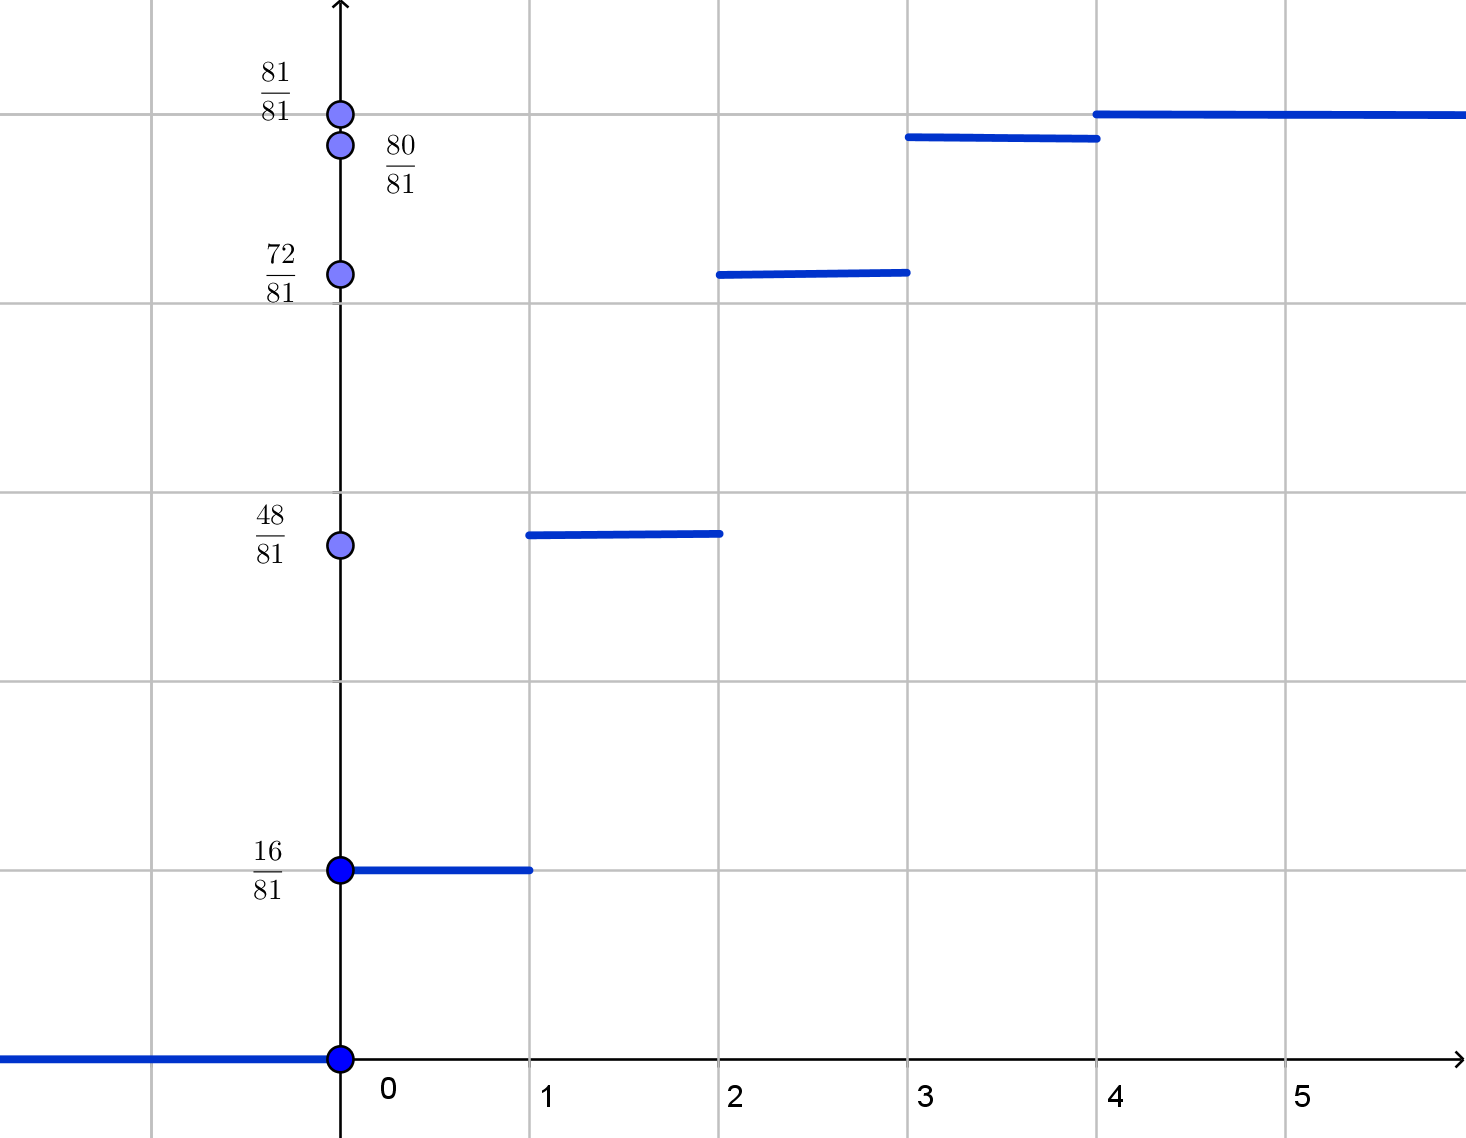
\includegraphics[width=80mm]{images/kr1_2017_3.png}
    }
    \caption{Функция распределения}
    \label{cdf_kr2017}
\end{figure}

\item Все вероятности посчитаны, видим, что наибольшая достигается при $\xi=1$.
\item $\E(X) = np = \frac{4}{3} $, $ \Var(X) = npq = \frac{8}{9}$
\end{enumerate}
\item
\begin{enumerate}
\item Так как указано, что цена сметаны распределена равномерно на отерзке $[250, 1000]$, максимальное значение цены — $1000$, это и есть необходимая сумма.
\item Вспомним, что функция распределения $F(x) = \P(X \leq x)$, нужно найти такой $x$, что $ \P(X \leq x)=0.9$:
\[
0.9 = 1 - \exp({-x^{2}}) \Rightarrow \exp(-x^{2}) = 0.1 \Rightarrow -x^2 = \ln(0.1)  \Rightarrow x=  \sqrt{-\ln(0.1)}
\]
\item Взяв производную от функции распределения списка без сметаны, получим функцию плотности:
\[
f_X(x) =
\begin{cases}
2x\exp(-x^2) & x \ge 0 \\
0 & \text{иначе}
\end{cases}
\]
Найдём математическое ожидание:
\[
\int_{0}^{+\infty}2x^2\exp({-x^2}) dx = -x \exp({-x^2})\big|_0^{+\infty} + \int_{0}^{+\infty}\exp({-x^2}) dx = \frac{\sqrt{\pi}}{2}
\]
\item Математическое ожидание суммы случайных величин равно сумме математических ожиданий случайных влечин, если они существуют. Математическое ожидание от цены сметаны равно: $ \frac{1000 + 250}{2} = 625 $
Математическое ожидание списка без сметаны было найдено в предыдущем пункте, его осталось перевести в рубли. Получаем ответ: $ 625 + \frac{\sqrt{\pi}}{2} \cdot 1000 $.
\item Так как обе величины имеют абсолютно непрерывные распределения, вероятность попасть в конкретную точку равна нулю.
\end{enumerate}
\item
\begin{enumerate}
\item $\P(\text{детектор показл ложь и подозреваемый лжёт}) = 0.9 \cdot 0.1 + 0.1 \cdot 0.95 = 0.185$
\item $\P(\text{невниовен}|\text{детектор показал ложь}) = \frac{0.9\cdot0.1}{0.185} = \frac{90}{185}$
\item $\P(\text{эксперт точно выявит преступника}) = (0.9)^9 \cdot 0.95$
\item $\P(\text{эксперт ошибочно выявит преступника}) = 9 \cdot 0.1 \cdot 0.9^8\cdot 0.05$
\end{enumerate}


%\item
%$\P(Ложь|Лжёт) = 0.95 $

%$\P(Ложь|Не лжёт) = 0.1 $

%$\P({Лжёт}) = \frac{1}{10} $

%\P(\text{Не лжёт}) = \dfrac{9}{10} $

%\begin{enumerate}
%	\item
%	По формуле полной вероятности: \[  \P(Ложь) = 0.95 \cdot 0.1 + 0.1 \cdot 0.9 = 0.185 \]
%	\item
%	По формуле Байеса: \[ \P(\text{Не лжёт}|Ложь) = \dfrac{0.1 \cdot 0.9}{0.185} = 0.486\]
%    \item
%    Событие "эксперт точно выявит преступника" соответствует событию "эксперт выявит, что лгун лжет, и      что остальные говорят правду".  Таким образом:  \[ \P = 0.1 \cdot 0.95 + 0.9 \cdot 0.9  = 0.905\]
%    \item
%    Это означает, что эксперт выберет 8 человек из 9 невиновных и скажет, что они говорят правду
%    (количество вариантов выбрать так людей  $С_9^8$ ), а также выберет 1 виновного и скажет, что он
%    говорит правду (количество вариантов это сделать 1), и выберет одного невиновного и скажет, что он
%    лжет (количество вариантов выбрать так человека $С_9^1$ ). Просуммируем все с учетом вероятностей,
%    указанных в условии: \[ \P = с_9^8 \cdot 0.9 \cdot 0.9 \cdot C_9^1 \cdot 0.9 \cdot 0.1 \cdot 1 \cdot 0.1
%    \cdot 0.05 = 0. 26244\]

%\end{enumerate}
\end{enumerate}



\subsection{Контрольная работа 1, ИП, 24.10.2017}


Ровно 272 года назад императрица Елизавета повелела завезти во дворцы котов для ловли мышей.


\begin{enumerate}

\item В отсутствии кота Леопольда мыши Белый и Серый подкидывают по очереди игральный додекаэдр
%\footnote{Леопольд подсказывает по случаю праздника, что у додекаэдра 12 граней :)}
.
Сыр достаётся тому, кто первым выкинет число 6. Начинает подкидывать Белый.

\begin{enumerate}
  \item Какова вероятность того, что сыр достанется Белому?
  \item Сколько в среднем бросков продолжается игра?
  \item Какова дисперсия числа бросков?
\end{enumerate}

\item Микки Маус, Белый и Серый решили устроить труэль из любви к мышки Мии. Сначала стреляет Микки, затем Белый, затем Серый, затем снова Микки и так до тех пор, пока в живых не останется только один.

Прошлые данные говорят о том, что Микки попадает с вероятностью $1/3$, Белый — с вероятностью $2/3$, а Серый стреляет без промаха.

Найдите оптимальную стратегию каждого мыша.

\item Микки Маус, Белый и Серый пойманый злобным котом Леопольдом до начала труэли. И теперь Леопольд будет играть с ними в странную игру.

В комнате три закрытых внешне неотличимых коробки: с золотом, серебром и платиной. Общаться после начала игры мыши не могут, но могут заранее договориться о стратегии.

Правила игры таковы. Кот Леопольд будет заводить мышей в комнату по очереди. Каждый из мышей может открыть
две коробки по своему выбору. Перед следующим мышом коробки закрываются.

Если Микки откроет коробку с золотом, Белый
— с серебром, а Серый — с платиной, то они выигрывают. Если
хотя бы один из мышей не найдёт свой металл, то Леопольд их съест.
\begin{enumerate}
\item Какова оптимальная стратегия?
\item Какова вероятность выигрыша при использовании оптимальной стратегии?
\end{enumerate}

\item Накануне войны Жестокий Тиран Мышь очень большой страны издал указ. Отныне за каждого новорождённого мыша-мальчика семья получает денежную премию, но если в семье рождается вторая мышка-девочка, то всю семью убивают. Бедные жители страны запуганы и остро нуждаются в деньгах, поэтому в каждой семье мыши будут появляться до тех пор, пока не родится первая мышка-девочка.

\begin{enumerate}
  \item Каким будет среднее число детей в мышиной семье?
  \item Какой будет доля мышей-мальчиков в стране?
  \item Какой будет средняя доля мышей-мальчиков в случайной семье?
  \item Сколько в среднем мышей-мальчиков в случайно выбираемой семье?
\end{enumerate}

\item Вальяжный кот Василий положил на счёт в банке на Гаити один гурд. Сумма на счету растёт непрерывно с постоянной ставкой в течение очень длительного промежутка времени. В случайный момент этого промежутка кот Василий закрывает свой вклад.

Каков закон распределения первой цифры полученной Василием суммы?

\begin{comment}
\item Начинающий трейдер Афанасий совершает не более одной сделки в день.

Если в какой-то день у трейдера Афанасия есть акция, то за этот день он равновероятно продаёт или не продаёт её. Если в какой-то день у трейдера Афанасия нет акций, то он равновероятно покупает или не покупает одну акцию.

Найдите ожидаемую прибыль Афанасия, если известно, что реализовывал он свою стратегию 100 дней, в начале акции стоили по 50 рублей, в конце — по 80 рублей, максимум составил 120 рублей, а минимум — 30.


\item Страшный Мейн-кун разрубает палочку единичной длины на $10$ частей в случайных и независимых местах, равномерно распределённых по всех длине. Затем Страшный Мейн-кун выбирает случайно один из кусочков и возводит его длину в $24$ степень.

Какое в среднем число он получит?
\end{comment}



\subsection{Контрольная работа 1, ИП, 24.10.2017, решения}


\begin{enumerate}

\item[1.]

\begin{enumerate}
	\item Обозначим вероятность того, что сыр достанется Белому за $b$, если игра начинается с его броска. Получаем уравнение
\[
	b = \frac{1}{12} + \frac{11}{12} \frac{11}{12} b
\]

Пояснение: Как Белый может победить в исходной игре? Либо сразу выкинуть 6 с вероятностью $1/12$. Либо передать ход Серому ($11/12$), получить ход снова ($11/12$) и выиграть в продолжении игры. Продолжение игры по сути совпадает с исходной игрой.

\item Игра продолжается до тех пор, пока кто-то не выкинет «6». Для нахождения среднего количества бросков воспользуемся методом первого шага.

Обозначим среднее количество бросков нашей игры за $S$. Когда Белый бросает кубик, с вероятностью $\frac{1}{12}$ игра закончится за один бросок, а с вероятностью $\frac{11}{12}$ игра продолжится и ход перейдёт к Серому. Но та игра, которая начнётся, когда бросать будет Серый, ничем не отличается от предыдущей, поэтому среднее количество бросков в ней будет равно $S$. Однако мы попадём в эту игру, «потратив» один бросок. Таким образом мы получаем:

\[
S = \frac{1}{12} \cdot 1 + \frac{11}{12}(S +1)
\]

Получается, что $S = 12$, значит игра длится в среднем 12 бросков.
\end{enumerate}

\item[3.]

Для того, чтобы выжить, мышам нужно ещё до начала игры договориться о стратегии, которая позволит им с наибольшей вероятностью открыть нужные сундуки. Если хотя бы две мыши выберут одинаковый сундук, то их в любом случае съедят. Поэтому одной из оптимальных стратегий будет ещё до начала игры мышам договориться и назвать левый сундук золотым, сундук посередине серебряным, а правый — платиновым. Каждый мышонок должен открыть тот сундук, в честь которого назван необходимый ему металл. Если внутри он обнаруживает свой металл, то он выбирает этот сундук, если внутри находится не тот металл, мышонок открывает тот сундук, на который указывает лежащий внутри предмет.

Например, первым заходит Микки Маус. Он открывает золотой (левый) ящик. Если внутри лежит золото, то он выходит из комнаты. Если же внутри лежит, например, серебро, то Микки Маус открывает сундук посередине. Путём несложного перебора можно посчитать, что в 4 случаях из 6 мыши смогут найти нужный металл, поэтому вероятность выигрыша при данной стратегии равна $\frac{2}{3}$.

\item[5.]

Функция распределения дохода кота Василия, положившего один гурд на вклад, представляется в виде $m_t = 1\cdot e^{rt}$, где $r$ — процентная ставка, а $t$ — прошедшее время. Момент закрытия вклада Т равномерно распределён на отрезке от 0 до $a$, который очень велик, поэтому сумма, которую получит Василий, представима в виде $Z = e^{Y}$, где $Y \sim v[0; ra]$.

Вероятность того, что первая цифра будет равна 1, равна вероятности того, что доход Василия будет лежать в пределах от 1 до 2 гурдов, плюс вероятность того, что он лежит в пределах от 10 до 20 гурдов и т.д. Таким образом, можно представить эту вероятность, как:
\[
\P(N=1) = \P(e^Y \in [1;2) ) + \P(e^Y \in [10; 20) ) + \ldots
\]

Это выражение можно преобразовать таким образом:
\[
\P(N=1) = \P(Y \in [\ln 1; \ln2) ) + \P(Y \in [\ln 10; \ln 20) ) + \ldots
\]

Так как Y — равномерно распределённая величина, то $\P(Y \in [\ln 1; \ln2) ) = \frac{\ln 2 - \ln 1}{ra}$. Для последующих слагаемых вероятность рассчитывается таким же образом. Воспользовавшись свойством логарифма, можно заметить, что $\frac{\ln 20 - \ln 10}{ra} = \frac{\ln 2}{ra}$. Поэтому вероятность того, что на первом месте суммы вклада стоит единица, равна $n\cdot \frac{\ln 2}{ra}$, где $n$ -- количество слагаемых. Путём аналогичных рассуждений получаем, что вероятность того, что на первом месте стоит двойка, равна $n\cdot \frac{\ln 3- \ln 2}{ra}$. Из-за того, что $a$ велико, можно считать, что число слагаемых одинаково.

Т.к. на первом месте обязательно будет находиться какая-то цифра, то сумма вероятностей будет равна 1. Получаем:
\[
\dfrac{n}{ra}(\ln \frac{2}{1} + \ln \frac{3}{2} + \ldots + \ln \frac{10}{9}) = 1
\]

Таким образом $\frac{n}{ra} = \frac{1}{\ln 10}$. Получается, что вероятность того, что на первом месте стоит единица, равна:
\[
\P (N=1) = \dfrac{\ln 2}{\ln 10}
\]

Закон распределения первой цифры выводится сложением соответствующих вероятностей.

\end{enumerate}
\end{enumerate}



\subsection{Теоретический минимум к кр2}

\begin{enumerate}
\item Сформулируйте определение независимости событий, формулу полной вероятности.
\item Приведите определение условной вероятности случайного события, формулу Байеса.
\item Сформулируйте определение и свойства функции распределения случайной величины.
\item Сформулируйте определение и свойства функции плотности случайной величины.
\item Сформулируйте определение и свойства математического ожидания для абсолютно непрерывной случайной величины.
\item Сформулируйте определение и свойства математического ожидания для дискретной случайной величины.
\item Сформулируйте определение и свойства дисперсии случайной величины.
\item Сформулируйте определения следующих законов распределений: биномиального, Пуассона, шеометрического, равномерного, экспоненциального, нормального. Укажите математическое ожидание и дисперсию.
\item Сформулируйте определение функции совместного распределения двух случайных величин, независимости случайных величин. Укажите, как связаны совместное распределение и частные распределения компонент случайного вектора.
\item	Сформулируйте определение и свойства совместной функции плотности двух случайных величин, сформулируйте определение независимости случайных величин.
\item Сформулируйте определение и свойства ковариации случайных величин.
\item Сформулируйте определение и свойства корреляции случайных величин.
\item Сформулируйте определение и свойства условной функции плотности.
\item Сформулируйте определение  условного математического ожидания $\E(Y|X=x)$ для совместного дискретного и совместного абсолютно непрерывного распределений.
\item Сформулируйте определение математического ожидания и ковариационной матрицы случайного вектора и их свойства.
\item Сформулируйте неравенство Чебышёва и неравенство Маркова.
\item Сформулируйте закон больших чисел в слабой форме.
\item Сформулируйте центральную предельную теорему.
\item Сформулируйте теорему Муавра—Лапласа.
\item Сформулируйте определение сходимости по вероятности для последовательности случайных величин.

\end{enumerate}


\subsection{Задачный минимум кр 2}

\begin{enumerate}

\item Пусть задана таблица совместного распределения случайных величин $X$ и $Y$.

\begin{center}\begin{tabular}{lccc}
\toprule
 $X$ \textbackslash $Y$    & $-1$  & $0$   & $1$   \\ \midrule
$-1$                 & $0.2$ & $0.1$ & $0.2$ \\
 $1$                 & $0.1$ & $0.3$ & $0.1$ \\ \bottomrule
\end{tabular}\end{center}


Найдите
\begin{enumerate}
\item $\P(X = -1)$
\item $\P(Y = -1)$
\item $\P(X = -1 \cap Y = -1 )$
\item Являются ли случайные величины $X$ и $Y$ независимыми?
\item $F_{X,Y}(-1,0)$
\item Таблицу распределения случайной величины $X$
\item Функцию $F_{X}(x)$ распределения случайной величины $X$.
\item Постройте график функции $F_{X}(x)$ распределения случайной величины $X$.
\end{enumerate}

\item Пусть задана таблица совместного распределения случайных величин $X$ и $Y$.


\begin{center}\begin{tabular}{lccc}
\toprule
 $X$ \textbackslash $Y$    & $-1$  & $0$  & $1$   \\ \midrule
$-1$                 & $0.2$ & $0.1$ & $0.2$ \\
 $1$                 & $0.2$ & $0.1$ & $0.2$ \\ \bottomrule
\end{tabular}\end{center}

Найдите
\begin{enumerate}
\item $\P(X = 1)$,
\item $\P(Y = 1)$,
\item $\P(X = 1 \cap Y = 1)$
\item Являются ли случайные величины $X$ и $Y$ независимыми?
\item $F_{X,Y}(1,0)$
\item Таблицу распределения случайной величины $Y$
\item Функцию $F_{Y}(y)$ распределения случайной величины $Y$
\item Постройте график функции $F_{Y}(y)$ распределения случайной величины $Y$.
\end{enumerate}

\item Пусть задана таблица совместного распределения случайных величин $X$ и $Y$.

\begin{center}\begin{tabular}{lccc}
\toprule
 $X$ \textbackslash $Y$    & $-1$  & $0$   & $1$   \\ \midrule
$-1$                 & $0.2$ & $0.1$ & $0.2$ \\
 $1$                 & $0.1$ & $0.3$ & $0.1$ \\ \bottomrule
\end{tabular}\end{center}

Найдите
\begin{enumerate}
    \item $\E(X),$
    \item $\E(X^{2}),$
	\item $\Var(X),$
    \item $\E(Y),$
    \item $\E(Y^{2}),$
    \item $\Var(Y),$
    \item $\E(XY),$
	\item $\Cov(X,Y)$
    \item $\Corr(X,Y)$
    \item Являются ли случайные величины $X$ и $Y$ некоррелированными?
\end{enumerate}

\item Пусть задана таблица совместного распределения случайных величин $X$ и $Y$.

\begin{center}\begin{tabular}{lccc}
\toprule
 $X$ \textbackslash $Y$    & $-1$  &$ 0 $  & $1 $  \\ \midrule
$-1$                 & $0.2$ & $0.1$ & $0.2$ \\
 $1$                 & $0.2$ & $0.1$ & $0.2$ \\ \bottomrule
\end{tabular}\end{center}

Найдите
\begin{enumerate}
    \item $\E(X),$
    \item $\E(X^{2}),$
	\item $\Var(X),$
    \item $\E(Y),$
    \item $\E(Y^{2}),$
    \item $\Var(Y),$
    \item $\E(XY),$
	\item $\Cov(X,Y)$
    \item $\Corr(X,Y)$
    \item Являются ли случайные величины $X$ и $Y$ некоррелированными?
\end{enumerate}

\item
Пусть задана таблица совместного распределения случайных величин $X$ и $Y$.

\begin{center}\begin{tabular}{lccc}
\toprule
 $X$\textbackslash $Y$    & $-1$  & $0$   & $1$   \\ \midrule
$-1$                 & $0.2$ & $0.1$ & $0.2$ \\
 $1$                 & $0.1$ & $0.3$ & $0.1$ \\ \bottomrule
\end{tabular}\end{center}

Найдите
\begin{enumerate}
\item $\P(X = -1 | Y = 0)$
\item $\P(Y = 0 | X = -1)$
\item таблицу условного распределения случайной величины $Y$ при условии $X = -1$
\item условное математическое ожидание случайной величины $Y$ при $X = -1$
\item условную дисперсию случайной величины $Y$
при условии $X = -1$
\end{enumerate}

\item Пусть задана таблица совместного распределения случайных величин $X$ и $Y$.

\begin{center}\begin{tabular}{lccc}
\toprule
 $X$ \textbackslash $Y$    & $-1$  & $0$   & $1$   \\ \midrule
$-1$                 & $0.2$ & $0.1$ & $0.2$ \\
 $1$                 & $0.2$ & $0.1$ & $0.2$ \\ \bottomrule
\end{tabular}\end{center}

Найдите
\begin{enumerate}
\item $\P(X = 1 | Y = 0)$
\item $\P(Y = 0 | X = 1)$
\item таблицу условного распределения случайной величины $Y$ при условии $X = 1$
\item условное математическое ожидание случайной величины $Y$ при $X = 1$
\item условную дисперсию случайной величины $Y$
при условии $X = 1$
\end{enumerate}

\item Пусть $\E(X)=1$, $\E(Y)=2$, $\Var(X) = 3$, $\Var(Y) = 4$, $\Cov(X,Y) = -1$. Найдите
\begin{enumerate}
\item $\E(2X + Y - 4)$
\item $\Var(3Y + 3)$
\item $\Var(X - Y)$
\item $\Var(2X - 3Y +1)$
\item $\Cov(X+ 2Y + 1,3X - Y -1)$
\item $\Corr(X + Y, X - Y)$
\item Ковариационную матрицу случайного вектора $Z = (X\hspace*{0.4cm} Y)$ \end{enumerate}


\item Пусть $\E(X)=-1$, $\E(Y)=2$, $\Var(X) = 1$, $\Var(Y) = 2$, $\Cov(X,Y) = 1$. Найдите
\begin{enumerate}
\item $\E(2X + Y - 4)$
\item $\Var(2Y + 3)$
\item $\Var(X - Y)$
\item $\Var(2X - 3Y +1)$
\item $\Cov(3X+ Y + 1,X - 2Y -1)$
\item $\Corr(X + Y, X - Y)$
\item Ковариационную матрицу случайного вектора $Z = (X\hspace*{0.4cm}Y)$
\end{enumerate}

\item Пусть случайная величина $X$ имеет стандартное нормальное распределение.

Найдите
\begin{enumerate}
\item $\P(0 < X < 1)$
\item $\P(X > 2)$
\item $\P(0 < 1 - 2X \leq 1)$
\end{enumerate}

\item Пусть случайная величина $X$ имеет стандартное нормальное распределение.

Найдите
\begin{enumerate}
\item $\P(-1 < X < 1)$
\item $\P(X < -2)$
\item $\P(-2 < -X + 1 \leq 0)$
\end{enumerate}

\item Пусть случайная величина $X \sim \cN(1,4)$. Найдите $\P(1<X<4)$

\item Пусть случайная величина $X \sim \cN(2,4)$. Найдите $\P(-2<X<4)$

\item Случайные величины $X$ и $Y$ независимы и  имеют нормальное распределение, $\E(X) = 0 $, $\Var(X) = 1$, $\E(Y) = 2$, $\Var(Y) = 6$. Найдите $\P(1 < X + 2Y < 7)$.

\item Случайные величины $X$ и $Y$ независимы и  имеют нормальное распределение, $\E(X) = 0 $, $\Var(X) = 1$, $\E(Y) = 3$, $\Var(Y) = 7$. Найдите $\P(1 < 3X + Y < 7)$.

\item Игральная кость подбрасывается $420$ раз. При помощи центральной предельной теоремы приближенно найти вероятность того, что суммарное число очков будет находиться в пределах от $1400$ до $1505$?

\item При выстреле по мишени стрелок попадает в десятку с вероятностью $0.5$, в девятку – $0.3$, в восьмерку – $0.1$, в семерку – $0.05$, в шестерку – $0.05$.
Стрелок сделал $100$ выстрелов. При помощи центральной предельной теоремы приближенно найти вероятность того, что он набрал не менее 900 очков?

\item Предположим, что на станцию скорой помощи поступают вызовы, число которых распределено по закону Пуассона с параметром $\lambda = 73$, и в разные сутки их количество не зависит друг от друга. При помощи центральной предельной теоремы приближенно найти вероятность того, что в течение года (365 дней) общее число вызовов будет в пределах от $26500$ до $26800$.

\item Число посетителей магазина (в день) имеет распределение Пуассона с математическим ожиданием $289$. При помощи центральной предельной теоремы приближенно найти вероятность того, что за $100$ рабочих дней суммарное число посетителей составит от $28550$ до $29250$ человек.

\item Пусть плотность распределения случайного вектора $(X,Y)$ имеет вид
\begin{center} $f_{X,Y}(x,y) = \begin{cases} x+y, & \text{при } (x,y) \in [0;1] \times [0;1] \\ 0 , & \text{при } (x,y) \not\in [0;1] \times [0;1] \end{cases}$  \end{center}

Найдите
\begin{enumerate}
\item $\P(X \leq \frac{1}{2} \cap Y \leq \frac{1}{2})$,
\item $\P(X\leq Y)$,
\item $f_{X}(x)$,
\item $f_{Y}(y)$,
\item Являются ли случайные величины $X$ и $Y$ независимыми?
\end{enumerate}

\item Пусть плотность распределения случайного вектора $(X,Y)$ имеет вид
\begin{center} $f_{X,Y}(x,y) = \begin{cases} 4xy, & \text{при } (x,y) \in [0;1] \times [0;1] \\ 0 , & \text{при } (x,y) \not\in [0;1] \times [0;1] \end{cases}$  \end{center}

Найдите
\begin{enumerate}
\item $\P(X \leq \frac{1}{2} \cap Y \leq \frac{1}{2})$,
\item $\P(X\leq Y)$,
\item $f_{X}(x)$,
\item $f_{Y}(y)$,
\item Являются ли случайные величины $X$ и $Y$ независимыми?
\end{enumerate}

\item Пусть плотность распределения случайного вектора $(X,Y)$ имеет вид
\begin{center} $f_{X,Y}(x,y) = \begin{cases} x+y, & \text{при } (x,y) \in [0;1] \times [0;1] \\ 0 , & \text{при } (x,y) \not\in [0;1] \times [0;1] \end{cases}$  \end{center}

Найдите
\begin{enumerate}
\item $\E(X)$,
\item $\E(Y)$,
\item $\E(XY)$,
\item $\Cov(X,Y)$,
\item $\Corr(X,Y)$.
\end{enumerate}

\item Пусть плотность распределения случайного вектора $(X,Y)$ имеет вид
\begin{center} $f_{X,Y}(x,y) = \begin{cases} 4xy, & \text{при } (x,y) \in [0;1] \times [0;1] \\ 0 , & \text{при } (x,y) \not\in [0;1] \times [0;1] \end{cases}$  \end{center}

Найдите
\begin{enumerate}
\item $\E(X)$,
\item $\E(Y)$,
\item $\E(XY)$,
\item $\Cov(X,Y)$,
\item $\Corr(X,Y)$.
\end{enumerate}

\item Пусть плотность распределения случайного вектора $(X,Y)$ имеет вид
\begin{center} $f_{X,Y}(x,y) = \begin{cases} x+y, & \text{при } (x,y) \in [0;1] \times [0;1] \\ 0 , & \text{при } (x,y) \not\in [0;1] \times [0;1] \end{cases}$  \end{center}

Найдите
\begin{enumerate}
\item $f_{Y}(y)$,
\item $f_{X|Y}\left(x|\frac{1}{2}\right)$
\item $\E\left(X|Y = \frac{1}{2}\right)$
\item $\Var\left(X|Y = \frac{1}{2}\right)$
\end{enumerate}

\item Пусть плотность распределения случайного вектора $(X,Y)$ имеет вид
\begin{center} $f_{X,Y}(x,y) = \begin{cases} 4xy, & \text{при } (x,y) \in [0;1] \times [0;1] \\ 0 , & \text{при } (x,y) \not\in [0;1] \times [0;1] \end{cases}$  \end{center}

Найдите
\begin{enumerate}
\item $f_{Y}(y)$,
\item $f_{X|Y}\left(x|\frac{1}{2}\right)$
\item $\E\left(X|Y = \frac{1}{2}\right)$
\item $\Var\left(X|Y = \frac{1}{2}\right)$
\end{enumerate}

\end{enumerate}

\subsection*{Ответы}

\begin{enumerate}

\item
\begin{enumerate}
\item   $0.5 $
\item   $0.3$
\item   $0.2$
\item   нет
\item   $0.3$
\item
\begin{tabular}{lrr}
\toprule
$X$ & $-1$  & $1$   \\ \midrule
$\P(\cdot)$ & $0.5$ & $0.5$ \\ \bottomrule
\end{tabular}
\item  $F_{X}(x) = \begin{cases}
0, & \text{при } x < -1 \\
0.5 , & \text{при } x \in [-1;1) \\
1, & \text{при }  x \geq 1
\end{cases}$
\end{enumerate}
\item
\begin{enumerate}
\item   $0.5$
\item   $0.4$
\item   $0.2$
\item   да
\item   $0.6$
\item
\begin{tabular}{lrrr}
\toprule
$Y$ & $-1$  & $0$   & $1$   \\ \midrule
$\P(\cdot)$ & $0.4$ & $0.2$ & $0.4$ \\ \bottomrule
\end{tabular}
\item   $F_{Y}(y) = \begin{cases}
0, & \text{при } y < -1 \\
0.4 , & \text{при } y \in [-1;0) \\
0.6, & \text{при }  y \in [0;1)\\
1, & \text{при } y \geq 1
\end{cases}$
\end{enumerate}

\item
\begin{enumerate}
\item   $0$
\item   $1$
\item  $1$
\item   $0$
\item   $0.6$
\item   $0.6$
\item   $0$
\item   $0$
\item   $0$
\item   да, являются некоррелированными, но нельзя утверждать, что являются независимыми
\end{enumerate}

\item
\begin{enumerate}
\item   $0$
\item   $1$
\item   $1$
\item   $0$
\item   $0.8$
\item   $0.8$
\item   $0$
\item   $0$
\item   $0$
\item   да, являются некоррелированными, но нельзя утверждать, что являются независимыми
\end{enumerate}

\item
\begin{enumerate}
\item   $0.25$
\item   $0.2$
\item   \begin{tabular}{lrrr}
\toprule
$Y$ | $\{X = -1\}$ & $-1$  & $0$   & $1$   \\ \midrule
$\P(\cdot)$              & $0.4$ & $0.2$ & $0.4$ \\ \bottomrule
\end{tabular}
\item   $0$
\item   $0.8 $
\end{enumerate}
\item
\begin{enumerate}
\item   $0.5$
\item   $0.2$
\item   \begin{tabular}{lrrr}
\toprule
$Y$ | $\{X = 1\}$ & $-1$  & $0$   & $1$   \\ \midrule
$\P(\cdot)$             & $0.4$ & $0.2$ & $0.4$ \\ \bottomrule
\end{tabular}
\item   $0$
\item   $0.8$
\end{enumerate}

\item
\begin{enumerate}
\item   $0 $
\item   $36$
\item  $9 $
\item   $60 $
\item  $-4$
\item   $\frac{-1}{3\sqrt{5}}$
\item  $\begin{pmatrix}
 3 & -1 \\
-1 & 4
\end{pmatrix}$
\end{enumerate}

\item
\begin{enumerate}
\item $-4$
\item $8 $
\item $1 $
\item $10 $
\item $-6$
\item$ \frac{-1}{\sqrt{5}}$

\item $\begin{pmatrix}
 1 & 1 \\
 1 & 2
\end{pmatrix}$
\end{enumerate}
\item
\begin{enumerate}
\item $0.3413$
\item $0.0228$
\item $0.1915$
\end{enumerate}

\item
\begin{enumerate}
\item $0.6826$
\item $0.0228  $
\item $0.1574  $
\end{enumerate}

\item $0.4332 $
\item $0.8185  $
\item $0.4514 $
\item $0.5328  $
\item $\approx 0.8185 $
\item $\approx 0.9115$
\item $\approx 0.6422 $
\item $\approx 0.9606$

\item
\begin{enumerate}
\item $0.125   $
\item $0.5 $
\item $f_{X}(x) = \begin{cases} x+\frac{1}{2}, & \text{при } x \in [0;1] \\ 0 , & \text{при } x \not\in [0;1] \end{cases}$
\item $f_{Y}(y) = \begin{cases} y+\frac{1}{2}, & \text{при } y \in [0;1] \\ 0 , & \text{при } y \not\in [0;1] \end{cases}$
\item нет
\end{enumerate}

\item
\begin{enumerate}
\item $\frac{1}{16}$

\item $\frac{1}{2}$

\item$f_{X}(x) = \begin{cases} 2x, & \text{при } x \in [0;1] \\ 0 , & \text{при } x \not\in [0;1] \end{cases}$

\item$f_{Y}(y) = \begin{cases} 2y, & \text{при } y \in [0;1] \\ 0 , & \text{при } y \not\in [0;1] \end{cases}$

\item да
\end{enumerate}

\item
\begin{enumerate}
\item $\frac{7}{12}$

\item $\frac{7}{12}$

\item $\frac{1}{3}$

\item $-\frac{1}{144}$

\item $-\frac{1}{11}$
\end{enumerate}

\item
\begin{enumerate}
\item $\frac{2}{3}$

\item $\frac{2}{3}$

\item $\frac{4}{9}$

\item 0

\item 0
\end{enumerate}

\item
\begin{enumerate}
\item $f_{Y}(y) = \begin{cases} y+\frac{1}{2}, & \text{при } y \in [0;1] \\ 0 , & \text{при } y \not\in [0;1] \end{cases}$

\item $f_{X|Y}(x|\frac{1}{2}) = \begin{cases} x+\frac{1}{2}, & \text{при } x \in [0;1] \\ 0 , & \text{при } x \not\in [0;1] \end{cases}$

\item $\frac{7}{12}$

\item $\frac{11}{144}$
\end{enumerate}

\item
\begin{enumerate}
\item $f_{Y}(y) = \begin{cases} 2y, & \text{при } y \in [0;1] \\ 0 , & \text{при } y \not\in [0;1] \end{cases}$

\item $f_{X|Y}(x|\frac{1}{2}) = \begin{cases} 2x, & \text{при } x \in [0;1] \\ 0 , & \text{при } x \not\in [0;1] \end{cases}$

\item $\frac{2}{3}$

\item $\frac{1}{18}$
\end{enumerate}
\end{enumerate}

\subsection{Контрольная работа 2, базовый поток, 09.12.2017}



\subsubsection{Минимум}
% 2 + 4 + 14 + 16

\begin{enumerate}
\item Приведите определение условной вероятности случайного события, формулу Байеса.
\item Сформулируйте определение и свойства функции плотности случайной величины. 
\item Сформулируйте определение  условного математического ожидания $\E(Y|X=x)$ для совместного дискретного и совместного абсолютно непрерывного распределений.
\item Сформулируйте неравенство Чебышёва и неравенство Маркова.

\item Задана таблица совместного распределения случайных величин $X$ и $Y$.
\begin{center}
\begin{tabular}{lccc}
\toprule
                       & $Y=-1$  & $Y=0$   & $Y=1$   \\ 
 \midrule
$X=0$                 & $0.2$ & $0.1$ & $0.3$ \\
 $X=1$                 & $0.2$ & $0.1$ & $0.1$ \\ 
 \bottomrule
\end{tabular}
\end{center}


\begin{enumerate}
    \item Найдите $F_{X,Y}(0, 0)$;
    \item Найдите $\E(X)$, $\E(X^2)$, $\E(Y)$, $\E(Y^2)$;
    \item Найдите $\Var(X)$, $\Var(Y)$;
    \item Найдите $\Cov(X, Y)$, $\Corr(X, Y)$
\end{enumerate}    
\item Плотность распределения случайного вектора $(X,Y)$ имеет вид
\[
f_{X,Y}(x,y) = 
\begin{cases} 
\frac{4x+10y}{7}, & \text{при } (x,y) \in [0;1] \times [0;1] \\ 
0 , & \text{при } (x,y) \not\in [0;1] \times [0;1] \\
\end{cases}
\]

\begin{enumerate}
\item Найдите $\P(X \leq Y)$;
\item Найдите функцию плотности $f_X(x)$;
\item Найдите $\E(X)$, $\E(Y)$ и $\Cov(X, Y)$;
\item Являются ли случайные величины $X$ и $Y$ независимыми?
\end{enumerate} 


\end{enumerate}

\subsubsection{Задачи}

\begin{enumerate}[resume]

\item Статистика авиакомпании «А» за много лет свидетельствует о том, что 10\% людей, купивших билет на самолет, не являются на рейс. Авиакомпания продала 330 билетов на 300 мест.
\begin{enumerate}
\item Какова вероятность, что всем явившимся на рейс пассажирам хватит места?
\item Укажите наибольшее число билетов, которое можно продавать на 300 мест, чтобы случаи переполнения случались не чаще, чем на одном из десяти рейсов.
\end{enumerate}

\item Сегодня акция компании «Ух» стоит 1 рубль. Каждый день акция может с вероятностью 0.7 вырасти на 1\%, с вероятностью 0.2999 упасть на 1\% и с вероятностью 0.0001 обесцениться (упасть на 100\%).
\begin{enumerate}
\item Считая изменение цены акции независимыми, найдите математическое ожидание её стоимости через 20 торговых дней.
\item Найдите предел по вероятности среднего изменения цены акции в процентах на бесконечном промежутке времени (Ответ обоснуйте).
\item Найдите математическое ожидание цены акции на бесконечном промежутке времени.
\item Инвестор вложил все свои средства в акции компании «Ух». Найдите вероятность его разорения на бесконечном промежутке времени.
\end{enumerate}


\end{enumerate}




\subsection{Контрольная работа 2, базовый поток, решения}

\begin{enumerate}
\item[7.]
\begin{enumerate}
\item Всем хватит места, если число явившихся на рейс пассажиров ($X$) не превысит $300$,
то есть нужно найти $\P(X \leq 300)$. Найдём матожидание и дисперсию
случайной величины $X$:
\begin{align*}
\E(X) &= np = 330 \cdot 0.9 = 297 \\
\Var(X) &= np(1-p) = 330 \cdot 0.9 \cdot 0.1 = 29.7
\end{align*}
Теперь посчитаем нужную вероятность:
\[
\P(X \leq 300) = \P \left(\frac{X - 297}{\sqrt{29.7}} \leq \frac{300 - 297}{\sqrt{29.7}} \right) = \P(\cN(0,1) \leq 0.55) \approx 0.709
\]
\item Вероятность переполнения не должна превышать $0.1$:
\begin{align*}
&\P(X > 300) < 0.1 \\
&\P\left(\frac{X - 0.9 \cdot n}{\sqrt{0.9 \cdot 0.1 \cdot n}} > \frac{300 - 0.9 \cdot n}{\sqrt{0.9 \cdot 0.1 \cdot n}} \right) < 0.1 \\
&\frac{300 - 0.9 \cdot n}{\sqrt{0.9 \cdot 0.1 \cdot n}}  > 1.28 \\
&300 - 0.9n > 1.28 \cdot 0.3 \sqrt{n} \\
&n < 325.6
\end{align*}
\end{enumerate}
\item[8.]
\begin{enumerate}
\item Выпишем случайную величину $X_i$ — цену акции после $i$-ого дня:
\[
X_i =
\begin{cases}
1.01, & p = 0.7 \\
0.99, & p = 0.2999 \\
0, & p = 0.0001
\end{cases}
\]
Нужно посчитать ожидание цены акциии после 20 дней:
\[
\E(X_1 \cdot \ldots \cdot X_{20}) \stackrel{\text{незав-ть}}{=} \E(X_1) \cdot \ldots \cdot \E(X_{20}) = 1.004^{20} \approx 1.083
\]
\item По ЗБЧ:
\[
\plim_{n\to\infty} \frac{1}{n} \sum_{i=1}^n X_i = \E(X_i) = 1.004
\]
\item Аналогично пункту (а):
\[
\E(X_1 \cdot \ldots \cdot X_{n}) = (\E(X_1))^n = 1.004^n
\]
И понятно, что $1.004^n \to_{n\to\infty} +\infty$.
\item
\begin{multline*}
\P(\text{разорения}) = 1 - \P(X_1 > 0, \ldots, X_n >0) = 1 - \prod_{i=1}^n \P(X_i > 0) \\
= 1 - (1 - 0.0001)^n \to_{n\to\infty} 1
\end{multline*}
\end{enumerate}
\end{enumerate}


\subsection{Кр2 — ИП часть}

\subsubsection{Тур 1}

\subsubsection{Тур 1 — Основная часть — Дискретные распределения}

\begin{enumerate}
% тур 1 - основная часть - дискретные распределения
\begin{problem}
\item[A1.] После смерти Мориарти на крыше Шерлоку нужно срочно вспомнить заранее обговорённое для такого исхода кодовое слово. Однако Шерлок так расстроился от смерти Джима, что совсем забыл то самое слово! К счастью, у Шерлока есть чертоги разума, в которых есть картинка кодового слова, но, почему-то, на греческом: \textbf{Λάζαρος} . К сожалению, Шерлок не изучал теорию вероятностей на экономе Вышки и плохо помнит греческий алфавит, вероятность вспомнить аналог буквы на латинице равна $0.8$, а раскладку на своём Blackberry он поменять не может.

\begin{enumerate}
\item Напишите кодовое слово русскими буквами.
\item Найдите вероятность того, что Шерлок отправит неправильное смс и не спасётся.
\end{enumerate}
\begin{sol}
\textbf{Внимание! Это задача-сюрприз!} Забираем в студию, если задача решена неверно.

Лазарос (Лазарь), $1-0.8^7$
\end{sol}
\end{problem}

% тур 1 - основная часть - дискретные распределения
\begin{problem}
\item[A2.] Мориарти объявил начало «Большой игры» — в течение $n$ дней каждый день его криминальными бандами будет свершаться преступление с вероятностью $p$ (независимо друг от друга). Бравые детективы Шерлок и Джон раскрывают каждое преступление с вероятностью $r$ (тоже независимо от предыдущих дней).
\begin{enumerate}
\item Найдите функцию распределения количества совершенных преступлений.
\item Найдите функцию распределения количества раскрытых преступлений. 
\end{enumerate}

\begin{sol}
$\P(X = k) = C^{\ k}_{\ n} (p)^k(1-p)^{n-k}$, \ $\P(Y = k) = C^{\ k}_{\ n}  (pr)^k(1-rp)^{n-k}$
\end{sol}
\end{problem}

% тур 1 - основная часть - дискретные распределения
\begin{problem}
\item[A3.]
Шерлок и Джон соперничают всю неделю и хотят выяснить, кто быстрее догадывается о личности настоящего убийцы. Пусть выигрывает тот, кто первым отгадал убийцу 4 раза подряд. $p$ — вероятность, что Джон оказался догадливее Шерлока и в конкретном деле быстрее вычислил виновного. Найдите вероятность того, что Джон выиграл во всей игре.

\begin{sol}
$\P(\text{Джон выигрывает}) = C^4_7p^4q^3 +C^5_7p^5q^2+C^6_7p^6q+p^7$ 
\end{sol}
\end{problem}

% тур 1 - основная часть - дискретные распределения
\begin{problem}
\item[A4.]
Ирэн и Шерлок очень любят писать друг другу смски, но стесняются показать свою привязанность. Шерлок подбрасывает монетку $n$ раз, а Ирэн — $n + 1$ раз. Оба придерживаются следующей стратегии: когда выпадает орёл, он/она отправляют смску, когда решка — ничего не отправляют. Найдите вероятность того, что Ирэн отправила больше смсок, чем Шерлок.

\begin{sol}
$1/2$
\end{sol}
\end{problem}

% тур 1 - основная часть - дискретные распределения
\begin{problem}
\item[A5.]
Шерлок пытается найти нужную информацию в чертогах разума. Пусть он находит её с вероятностью $p$ за одну попытку и не находит с вероятностью $q=1 -p$. $X$ — число попыток, которое понадобилось Шерлоку. Найдите $\E\left(\frac{1}{X+1} \right)$.

\begin{sol}
$- \frac{p}{q} \ln p$
\end{sol}
\end{problem}




\end{enumerate}

\newpage
\subsubsection{Тур 1 — Основная часть — Комбинаторика}

\begin{enumerate}

% тур 1 - основная часть - комбинаторика
\begin{problem}
\item[B1.] ОБН прослушивает телефон Джесси Пинкмана, поэтому он решил отправить закодированное послание мистеру Уайту, чтобы сохранить в секрете место следующей встречи. Для дополнительной секретности он составляет текст на русском языке, а потом кодирует каждую букву последовательностью из нулей и единиц длины $n$. Он хочет отправить послание как можно скорее и исключить неоднозначность раскодирования, поэтому выбирает наименьшее подходящее $n$. Чему оно равно?

\begin{sol}
$6$
\end{sol}
\end{problem}

% тур 1 - основная часть - комбинаторика
\begin{problem}
\item[B2.] Хэнк и Уолтер решили сыграть в следующую игру: каждый по очереди называет такую расстановку пяти ладей на шахматной доске, что ни они не бьют друг друга. Начинает Хэнк. Сколько ходов возможно сделать в этой игре, если играть до самого конца, а повторять уже названные расстановки нельзя.

\begin{sol}
$64 \cdot 49 \cdot 36 \cdot25 \cdot 16$ или $45\,158\,400$
\end{sol}
\end{problem}

% тур 1 - основная часть - комбинаторика
\begin{problem}
\item[B3.] Вернемся к сюжету из первой задачи. Все понимают, что Джесси может иногда совершить ошибку, пока кодирует свое послание. Поэтому теперь мистер Уайт и Джесси хотят так кодировать символ, чтобы даже при совершении Джесси ошибки в одном знаке можно было правильно раскодировать символ. Какого $n$ им будет достаточно сейчас? 

\begin{sol}
\textbf{Внимание! Это задача-сюрприз!} Предлагаем на выбор: частичный балл за какую-нибудь задачу / освобождение участника из студии

$9$
\end{sol}
\end{problem}

% тур 1 - основная часть - комбинаторика — Клад!
\begin{problem}
\item[B4.] Уолт поспорил с сыном, сможет ли он расставить числа от 1 до 2016 по кругу так, чтобы все суммы соседних чисел были разными. Выиграет ли он в споре и почему?

\begin{sol}
\textbf{Ответ:} да, выиграет

\textbf{Решение:} Рассмотрим расстановку $1, 2, 3,\hdots, 2014, 2016, 2015$. Выпишем суммы соседних чисел: $1+2 = 3, 2+3 = 5, 3+4 = 7,\hdots, 2013+2014 = 4027, 2014+
2016 = 4030, 2016 + 2015 = 4029, 2015 + 1 = 2016$. В этом списке по одному
разу появятся нечетные числа $3, 5,\hdots, 4027, 4029$ и четные $4030, 2016$.
\end{sol}
\end{problem}

% тур 1 - основная часть - комбинаторика
\begin{problem}
\item[B5.] Уолт собирается оставить свой уличный бизнес одному из 3 бывших учеников. У первого ученика есть два наследника, у второго — три, а у третьего — пять. Всем известно, что Уолт скоро объявит, кто именно сменит его на уличном престоле. На какое наименьшее количество районов можно разделить город так, чтобы при любом выборе Уолта, новый властитель мог бы раздать все округа своим наследникам, и каждому из них досталась бы территория одинаковой площади?

\begin{sol}
8
\end{sol}
\end{problem}
\end{enumerate}



\newpage
\subsubsection{Тур 1 — Основная часть — Метод первого шага}

\begin{enumerate}
% тур 1 - основная часть - метод первого шага
\begin{problem}
\item[C1.] Джоуи решил посмотреть телевизор после очередных неудачных проб на роль в сериале. Сейчас по телевизору идут новости. Джоуи переключает каналы в поисках футбольного матча, при этом известно, что на каждом канале показывают футбол с вероятностью $p=0.7$ и новости с вероятностью $1-p=0.3$. Пусть $X -$ это количество каналов, которые посмотрел Джоуи, прежде чем нашёл футбольный матч. Найдите $\E(X), \E(X^2), \Var(X)$ методом первого шага.

\begin{sol}
$\frac{10}{7},\frac{130}{49},\frac{30}{49}$
\end{sol}
\end{problem}

% тур 1 - основная часть - метод первого шага
\begin{problem}
\item[C2.] Фиби и Чендлер решили посмотреть телевизор после ссоры с Джоуи. Они включают телевизор и видят, что сейчас как раз идет фильм с ним. Фиби переключает каналы в поисках мультиков, при этом при переключении каналов действует следующее правило: при нечётном переключении канала Фиби попадёт на мультики с вероятностью $p=0.5$ и на фильм с Джоуи с вероятностью $1-p=0.5$, а при чётном — с вероятностями $p=0.75$ и $1-p=0.25$ соответственно. Пусть $X$ — это количество каналов, которые посмотрела Фиби, прежде чем нашла мультики. Найдите $\E(X), \E(X^2), \Var(X)$ методом первого шага.

\begin{sol}
$\frac{12}{7},\frac{164}{49},\frac{20}{49}$
\end{sol}
\end{problem}

% тур 1 - основная часть - метод первого шага — Клад!
\begin{problem}
\item[C3.] Росс подкидывает правильную монетку. Если монетка выпадает орлом, Росс генерирует случайную величину $X\sim \cN(1,\sigma^2)$, если монетка выпадает решкой, Росс> подкидывает монетку заново. Если монетка на этот раз выпадает орлом, Чендлер генерирует случайную величину $X\sim \cN(\frac{1}{2},\frac{1}{4}\sigma^2)$, иначе подкидывает монетку заново. В общем случае если монетка выпадает орлом на $n$-тое подкидывание, Чендлер  генерирует случайную величину $X\sim \cN \left(\frac{1}{2^{n-1}},\frac{1}{4^{n-1}}\sigma^2 \right)$. Найдите $\E(X), \E(X^2)$ методом первого шага.

\begin{sol}
\textbf{Ответ:} $\frac{2}{3},\frac{4(\sigma^2+1)}{7}$

\textbf{Решение:} Заметим, что на $n$-том шаге случайную величину $X$ можно представить как: $X = \frac{1}{2^{n-1}}+\frac{1}{2^{n-1}}\sigma^\cdot\varepsilon,\;\; \varepsilon\sim \cN(0,1)$, поэтому
\[
\E(X)= 0.5\cdot \E(1+\sigma\cdot \cN(0,1)) + 0.5\cdot \E\left(\frac{X}{2}\right)   \rightarrow \E(X)=\frac{2}{3}
\]
\[
\E(X^2)= 0.5\cdot \E((1+\sigma\cdot \cN(0,1))^2) + 0.5\cdot \E\left(\frac{X^2}{4}\right)
\rightarrow \E(X^2)=\frac{4(\sigma^2+1)}{7}
\]
\[
(Z\sim \cN(\mu,\sigma^2)\rightarrow \E(Z^2)=\mu^2 + \sigma^2)
\]
\end{sol}
\end{problem}


% тур 1 - основная часть - метод первого шага
\begin{problem}
\item[C5.] На свадьбе у Рэйчел женская часть гостей выстроились в линию чтобы ловить букет. В линии в случайном порядке стоят $n$ девушек, все разного роста. Моника  опаздывает и не успевает встать в ряд, поэтому ей удаётся посмотреть на всю линию только сбоку. Сколько в среднем жаждущих выйти замуж девушек увидит Моника? 

\begin{sol}
$1+\frac{1}{2}+\dots+\frac{1}{n}$
\end{sol}
\end{problem}
\end{enumerate}

\newpage
\subsubsection{Тур 1 — Основная часть — Неравенства Чебышёва и Маркова}


\begin{enumerate}
% тур 1 – основная часть – неравенства
\begin{problem}
\item[D1.] Вы Раджеш Кутрапали и у вас проблемы в общении с девушками. Если вы не выпьете алкоголь, то вы не можете разговаривать с женщинами. Каждые пол минуты вы равновероятно делаете глоток пива или нет. Если вы сделаете более 25 глотков, то вы дойдёте до нужной кондиции. Оцените сверху вероятность того, что через 20 минут Раджеш сможет говорить с прекрасной половиной человечества. 

\begin{sol}
$\P(\text{Радж готов}=True) \leq 0.8$
\end{sol}
\end{problem}

% тур 1 – основная часть – неравенства
\begin{problem}
\item[D2.] Вы команда кафедры теоретической физики по страйкболу, вы должны защитить честь кафедры на чемпионате по страйкболу ведь в нём участвуют географы, биологи и, что самой ужасное, гуманитарии. В вашей команде четверо человек. В команде гуманитариев 6 человек. Говорят, что на одного павшего в страйкболе приходится в среднем 100 шариков. Сколько нужно вам взять шариков в среднем на человека, чтобы оценка сверху убийства не менее 6 человек в неравенстве Маркова была равна 1? Для простоты считайтйе, что вы все переживёте эту бойню.

\begin{sol}
\textbf{Внимание! Это задача-сюрприз!} Предлагаем на выбор: -5 минут от времени клада / -5 очков команде-сопернику

Не менее 150 на человека.
\end{sol}
\end{problem}

% тур 1 – основная часть – неравенства
\begin{problem}
\item[D3.] Вы Говард Воловиц инженер с всего лишь степенью магистра. Вы конструируете робота, у которого имеется 100 узлов, которые могут сломаться за время автономной работы с вероятностью в 10\%. Оцените сверху вероятность того, что число поломанных узлов будет отличаться от ожидаемого более чем на 5 узлов. 

\begin{sol}
$\P(\vert \text{Поломок} - \E(\text{Поломок}) \vert  >5) \leq 9/25$
\end{sol}
\end{problem}

% тур 1 – основная часть – неравенства
\begin{problem}
\item[D4.] Вы Пенни, весьма милая девушка без высшего образования. Но вы переобщались с Шелдоном Купером. Из-за этого в вашей голове возникла задачка. Вы знаете, что каждые 20 минут у вас на работе заказывают два сырника с вероятностью $1/4$ и с такой же не заказывают, с оставшейся вероятностью у вас берут один сырник. Ваша смена длится 6 часов. Вы хотите оценить сверху вероятность того, что у вас закажут более 24 или менее 12 сырников. 

\begin{sol}
$\P(\vert \text{Сырников за смену} - \E(\text{Сырников за смену}) \vert  >6) \leq 1/4$
\end{sol}
\end{problem}

% тур 1 – основная часть – неравенства
\begin{problem}
\item[D5.] Вы Бернадетт Мэри Энн Ростенковски-Воловиц, микробиолог и вы скрестили Эболу с гриппом, но этого не было. Вы знаете что за условный период времени число бактерий возрастает либо в 2.71 раз либо в 7.39 раз равновероятно. Оцените снизу вероятность того что число бактерий за 20 условных периодов возрастет от $e^{25}$ до $e^{35}$ раз.

\begin{sol}
$\P(e^{25} \leq \text{Рост} \leq e^{35}) \geq 0.8 $ 
\end{sol}
\end{problem}


\end{enumerate}

\newpage
\subsubsection{Тур 1 — Основная часть — Условные вероятности}

\begin{enumerate}
% тур 1 - основная часть - условные вероятности
\begin{problem}
\item[E1.] Мы знаем, что кроме Элевен в Национальной лаборатории Хоукинса были еще дети. Предположим, в самом начале экспериментов было двое детей, один из которых был мальчиком. Если предположить, что Доктор Бреннан мог похитить равновероятно мальчика или девочку, то какова вероятность, что второй ребенок тоже был мальчиком?

\begin{sol}
$\frac{1}{3}$
\end{sol}
\end{problem}

% тур 1 - основная часть - условные вероятности
\begin{problem}
\item[E2] Из 100 опрошенных жителей Хоукинса, 30 работают в Национальной лаборатории Хоукинса, из которых 10 знают о том, что был открыт проход на «ту сторону». Какова вероятность, что если опрошенный житель работает в лаборатории, то он знает о проходе?

\begin{sol}
$\frac{1}{3}$
\end{sol}
\end{problem}

% тур 1 - основная часть - условные вероятности
\begin{problem}
\item[E3.] Встретившись лицом к лицу с Демогоргном, Дастин Лукас и Майк используют против него единственное оружие, которое у них есть — рогатки. Все трое напуганы и стреляют независимо. Дастин попадает с вероятностью $\frac{1}{4}$, Майк — с вероятностью $\frac{1}{6}$, А Лукас — с вероятностью $\frac{1}{3}$.

\begin{enumerate}
\item Какова вероятность, что только один из них попадет в монстра?
\item Каковая вероятность, что попадет Лукас, если попал только один из ребят?
\end{enumerate}

\begin{sol}
a) $\frac{31}{72}$; б) $\frac{15}{31} $
\end{sol}
\end{problem}

% тур 1 - основная часть - условные вероятности
\begin{problem}
\item[E4.]  Дастин, Лукас, Майк и Уилл играют в Dungeons and Dragons в подвале у Майка. Из 25 игральных карт, дающих специальные способности, 5 карты дают рунные заклинания, которые помогут пройти сквозь лес с демодогами. Ребята вытягивают карты по очереди. У кого больше вероятность вытащить счастливый билет: у Уилла (он тянул первый), или Лукаса (тянул вторым)?

\begin{sol}
\textbf{Внимание! Это задача-сюрприз!} Предлагаем на выбор: стикеры / возможность открыть клетку, к которой нет пути (десант!)

$\P(L|W)=\frac{4}{24}, \P(L|W^{c})=\frac{5}{24}, \P(W)=\frac{1}{5}, \P(W^{c})=\frac{4}{5}$ \\
$\P(L)=\frac{4}{24}\frac{1}{5}+\frac{5}{24}\frac{4}{5} = \frac{1}{5}= \P(W)$. Вероятность одинаковая.
\end{sol}
\end{problem}

% тур 1 - основная часть - условные вероятности
\begin{problem}
\item[E5.] Дастин и Макс играют в игровые автоматы. Дневной матч состоит из серии игр, причем $p$ — вероятность Дастина выиграть каждую игру (независимо). Первый, кто выигрывает на две игры больше противника, становится победителем дня. Какова вероятность того, что Дастин выиграет дневной матч (в терминах $p$)?

\begin{sol}
$\P(D) = \frac{p^2}{1-2pq}=\frac{p^2}{p^2+q^2}$
\end{sol}
\end{problem}

\end{enumerate}




\newpage
\subsubsection{Тур 1 — студия — Ковариации и корреляции}

\begin{enumerate}

% тур 1 - студия - ковариации и корреляции
\begin{problem}
\item[A1.] Создатель правой палочки и создатель левой палочки Twix бросают одновременно правильный десятигранный шоколадный кубик. Пусть $X$ и $Y$ значения, которые выпали создателю правой и левой палочки соответственно.

Найдите ковариацию между $X+Y$ и $X-Y$.

\begin{sol}
$\Cov(X+Y,X-Y) = 0 $
\end{sol}
\end{problem}

% тур 1 - студия - ковариации и корреляции
\begin{problem}
\item[A2.] Вы пошли на интервью, для того, чтобы сниматься в рекламе Альпен Гольда. Вы очень понравились жюри, но они хотят проверить ваше знание статистики. Вам дают такую задачу.

Пусть $\E(X) = 3, \E(\lambda) = -2, \Var(X) = 1,\E(\lambda^2) = 8, \E(X\lambda) = -1$
Найдите $\Cov(X,\lambda), \Corr(X,\lambda)$

\begin{sol}
$\Cov(X,\lambda) = 5, \Corr(X,\lambda)= 2.5$.
\end{sol}
\end{problem}

% тур 1 - студия - ковариации и корреляции
\begin{problem}
\item[A3.] Верны ли следующие утверждения?

\begin{enumerate}
\item Некоррелированные нормально распределенные случайные величины независимы.
\item Случайные величины $X$ и $Y$ зависимы, $Y$ и $Z$ зависимы. Верно ли, что случайные величины $X$ и $Z$ зависимы?
\end{enumerate}

\begin{sol}
а) Нет, б) Нет
\end{sol}
\end{problem}

% тур 1 - студия - ковариации и корреляции
\begin{problem}
\item[A4.] Вы пытаетесь оценивать зависимость между продажами Сникерса и печенья. Вам известно количество продаж в $100$ магазинах (нарисованы на графике). По оси $OX$ количество проданных Сникерсов, по оси $OY$ продажи печенья. 

Существует ли зависимость между продажами Сникерса и печенья? Какой знак у корреляции? 

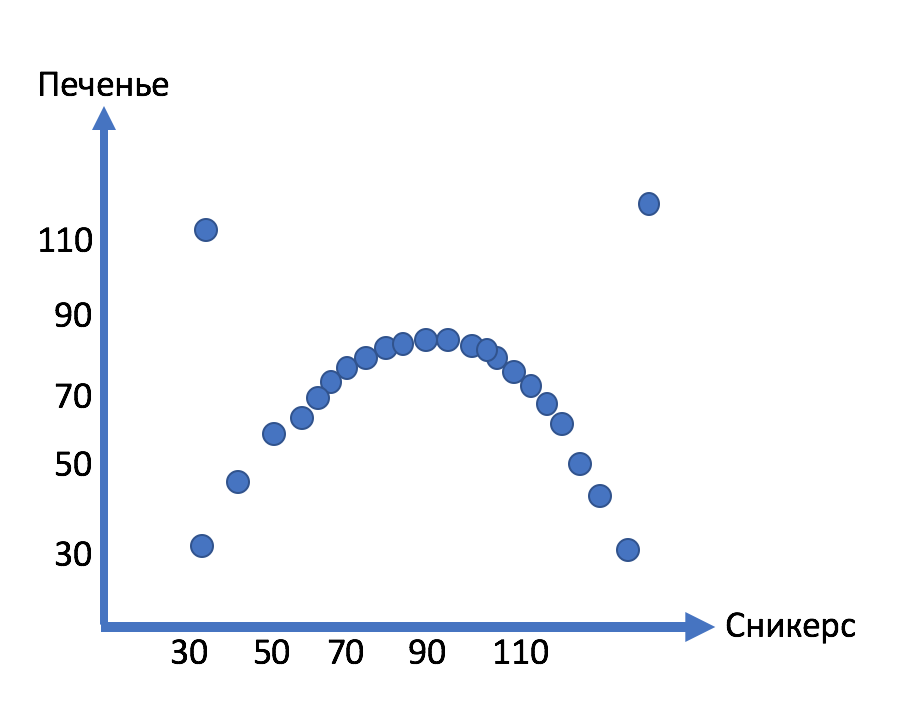
\includegraphics[scale=0.5]{images/No_correlation}

\begin{sol}
$X$ и $Y$ зависимы, но корреляция равна $0$.
\end{sol}
\end{problem}
\end{enumerate}


\newpage
\subsubsection{Тур 1 — студия — Нормальное распределение}

\begin{enumerate}
\begin{problem}
\item[B1.] Микрофинансовая организация «Рабочие деньги» обычно предлагает займы под \(144\%\) годовых. По случаю своего дня рождения она решила устроить акцию: для одного счастливчика ставка будет равна не \(144\%\) годовых, а реализации случайной величины \(X\sim \mathcal{N}(144; 1296)\). Найдите вероятность того, что ставка для счастливчика превысит \(180\%\) годовых.

\begin{sol}
$\approx 0.1586553$
\end{sol}
\end{problem}

\begin{problem}
\item[B2.] Директор «Рабочих денег» Иннокентий, пытается оценить, как распределены доходы его заёмщиков. Он считает, что распределение нормальное, но не уверен, какие у него параметры. Иннокентий нарисовал две функции распределения: $\cN(10000, 5000)$ и $\cN(12500, 15)$. Воспроизведите схематично рисунок Иннокентия.

\begin{sol}
$\cN(10000, 5000)$ — колокол, симметричный относительно прямой $x=10000$, с маленьким горбом; $\cN(12500, 15)$ — колокол, симметричный относительно прямой $x=12500$ с очень острым и узким горбом.
\end{sol}
\end{problem}

\begin{problem}
\item[B3.] На номер 8 800-555-35-35 поступил звонок от Валерия. Как хорошо, что Иннокентий заранее определился с распределением доходов своих клиентов! Доход каждого – случайная величина, распределённая нормально с математическим ожиданием $15000$. Проведя беглый опрос, Иннокентий прикинул вероятность того, что истинный доход Валерия лежит в интервале $(12000, 13000)$. По его оценке, она равна $0.3$. А какова вероятность того, что истинный доход Валерия лежит в интервале $(17000, 18000)$?

\begin{sol}
$0.3$
\end{sol}
\end{problem}

\begin{problem}
\item[B4.] Иннокентий снова делает квартальный отчёт. В этот раз он уверен, что распределение доходов заёмщиков – нормальное с матожиданием $20000$ и стандартным отклонением $1000$. Но он совсем забыл функцию плотности нормального распределения, поэтому написал смс жене: «Котя, напомни функцию плотности нормального распределения, плз». Помогите Иннокентию, плз.

\begin{sol}
$f(x) = \frac{1}{\sqrt{2 \pi 1000^2}}e^{-\frac{1}{2}\cdot \frac{(x-20000)^2}{1000^2}}$
\end{sol}
\end{problem}

\end{enumerate}


\newpage
\subsubsection{Тур 1 — студия — Непрерывные распределения}

\begin{enumerate}
% тур 1 - студия - непрерывные распределения
\begin{problem}
\item[C1.] Количество сиреневых конфет Skittles в каждой пачке – равномерная на отрезке $[0; \pi]$ случайная величина. Найдите $\P(\min\{X_1, \ldots, X_{1000}\} > e)$.

\begin{sol}
$\left(\frac{\pi - e}{\pi}\right)^{1000}$
\end{sol}
\end{problem}

% тур 1 - студия - непрерывные распределения
\begin{problem}
\item[C2.] Растаман в рекламе Skittles доит жирафа. Доля конфет красного цвета в надое – случайная величина и имеет следующую функцию распределения:

\[
F(x)  = \begin{cases}
C_1, & x < 0 \\
0.5 x^2 + 0.5x + C_3, & x\in [0,1] \\
C_2, & x > 1
\end{cases}
\]
Найдите $C_3$.

\begin{sol}
$0$
\end{sol}
\end{problem}

% тур 1 - студия - непрерывные распределения
\begin{problem}
\item[C3.] Количество сахара в граммах в конфете Skittles — случайная величина с функцией распределения $F(x) = \frac{1}{2} + \frac{\arctan(x)}{\pi}$. Найдите $\P(0<X<1)$.

\begin{sol}
$\frac{1}{4}$
\end{sol}
\end{problem}

% тур 1 - студия - непрерывные распределения
\begin{problem}
\item[C4.] Чтобы рассмотреть всю радугу, жирафу, стоящему прямо перед ней, нужно наклонять голову вправо или влево. Угол наклона головы – случайная величина $X$ с функцией плотности:

\[
f(x) = \begin{cases}
\frac{2}{\pi} \cos^2 x & x \in \left[-\frac{\pi}{2}, \frac{\pi}{2}\right] \\
0 & \text{иначе}
\end{cases}
\]

Жираф наклоняет трижды. Найдите вероятность того, что ровно два раза угол наклона будет лежать в интервале $\left(0, \frac{\pi}{4}\right)$.

\begin{sol}
$C_3^2 \left(\frac{2+\pi}{4\pi}\right)^2 \frac{3\pi-2}{4\pi}$
\end{sol}
\end{problem}
\end{enumerate}


\newpage
\subsubsection{Тур 1 — студия — Оптимальные стратегии}

\begin{enumerate}
% тур 1 - студия - оптимальные стратегии
\begin{problem}
\item[D1.] Леонид Якубович подбрасывает неправильную монетку и каждый раз пытается угадать, как она выпадет. В качестве прогноза на следующий бросок он использует результат предыдущего броска. Монетка выпадает орлом с вероятностью $p$.

Если Якубович угадывает, он получает от игрока Поле Чудес один евро, если не угадывает, то платит игроку один евро.

При каком $p$ стратегия Якубовича приносит игроку наибольшую ожидаемую прибыль? Чему она при этом будет равна?

\begin{sol}
D1. $E(X)=-1 + 4p(1-p)$. Максимизируем, получаем $p=0.5$. Наибольшая прибыль игрока $E(X)=0$.
\end{sol}
\end{problem}

% тур 1 - студия - оптимальные стратегии
\begin{problem}
\item[D2.] Леонид Якубович выдаёт шкатулки по новым правилам :) Деньги лежат только в одной из четырёх предлагаемых шкатулок. Марь-Ивановна из деревни Невероятная Глушь слышит:
— Вы, Марь-Ивановна, можете выбрать любую из четырёх шкатулок. Затем я открою одну пустую шкатулку (кроме Вашей) и снова дам Вам право выбора. Вы сможете сменить выбор шкатулки или настоять на прежнем. После этого, Марь-Ивановна, Вы получите содержимое шкатулки.

Как выглядит оптимальная стратегия Марь-Ивановны и чему равна вероятность выигрыша?

\begin{sol}
D2. Правильно будет сменить выбор. Вероятность удачи тогда будет равна $3/8$.
\end{sol}
\end{problem}

% тур 1 - студия - оптимальные стратегии
\begin{problem}
\item[D3.] Леонид Якубович подкидывает кубик. Если выпадает тройка, или Якубович говорит «стоп», то игра оканчивается, если нет, то начинается заново.
Выигрыш Леонид Аркадьевича - последнее выпавшее число. 

Как выглядит оптимальная стратегия и чему равен наибольший ожидаемый выигрыш?

\begin{sol}
D3. Говорить «стоп» на 3, 5, 6. Выигрыш равен $(3+5+6)/3=4+2/3$.
\end{sol}
\end{problem}


% тур 1 - студия - оптимальные стратегии
\begin{problem}
\item[D4.] Приз в Поле Чудес $X$ равномерно распределен от 0 до 1 миллиона рублей. Лингвист Вася имеет право заранее выбрать порог $b$. Если $X$ окажется больше порога $b$, то лингвист Вася получает $X$. Если $X$ окажется меньше порога $b$, то Вася не получает ничего.

Какой порог следует выбрать Василию?

\begin{sol}
D4. Очевидно 0, лучше всегда что-то получать :)
\end{sol}
\end{problem}
\end{enumerate}


\newpage
\subsubsection{Тур 2}

\subsubsection{Тур 2 — Основная часть — Непрерывные распределения}

\begin{enumerate}
% тур 2 - основная часть - непрерывные распределения
\begin{problem}
\item[A1.] Марта и Доктор заперты в старом особняке, куда их привела ТАРДИС. А еще в этом особняке заперты Плачущие Ангелы, передвигающиеся со скоростью $X$ м/с. Функция плотности величины $X$ имеет вид:
\[
f(t) = \begin{cases}
0, &  t<1 \\
t-a, & t \in [1,2) \\
0, & t \geq 2
\end{cases}
\]
Найдите $a$, $\E(X)$.

\begin{sol}
$a = \frac{1}{2}$, $\E(X) = \frac{19}{12}$
\end{sol}
\end{problem}

% тур 2 - основная часть - непрерывные распределения
\begin{problem}
\item[A2.] Сливины с планеты Раксакорикофаллапаториус и сонтаранцы с планеты Сонтар не могут решить, какой народ уродливее, и устраивают войну. Сонтар - планета воинов, у них преимущество в данной схватке. Пусть случайная величина $X$ - прибыль сонтаранцев от войны.  Функция плотности случайной величины $X$ имеет вид:
\[
f(x) = \begin{cases}
cx +3, & -3 \leq x \leq -2 \\
3-cx, & 2 \leq x \leq 3 \\
0, & \text{иначе}
\end{cases}
\]
Найдите константу $c$, функцию распределения случайной величины $X$.

\begin{sol}
\textbf{Внимание! Это задача-сюрприз!} Предлагаем на выбор: -5 минут от времени клада / -5 очков команде-сопернику

$c=1$, $F(x) = \begin{cases}
0, & x \leq -3 \\
\frac{(x+3)^2}{2}, & -3 \leq x < -2 \\
\frac{1}{2}, & -2 \leq x < 2 \\
1 - \frac{(x+3)^2}{2}, & 2 \leq x < 3 \\
1, & x \geq 3
\end{cases}
$
\end{sol}
\end{problem}

% тур 2 - основная часть - непрерывные распределения
\begin{problem}
\item[A3.] Всем известно, что ТАРДИС внутри на самом деле круглая. Пока Доктор спал, Эми решила наконец удовлетворить свое любопытство по поводу настоящего размера будки–машины времени и измерила ее диаметр $x$. $x$ измерен приближённо, причём $a \leq x \leq b$. Рассматривая диаметр как случайную величину $X$, распределённую равномерно в интервале $(a, b)$, найти математическое ожидание и дисперсию площади ТАРДИС.

\begin{sol}
$\frac{\pi(b^2 + ab + a^2)}{12}$, $\left(\frac{\pi^2}{720}\right) (b-a)^2 (4b^2 +7ab + 4a^2)$
\end{sol}
\end{problem}

% тур 2 - основная часть - непрерывные распределения
\begin{problem}
\item[A4.] Далеки считают, что вся сила Доктора заключена в его звуковой отвертке единичной длины. Предводитель Далеков Даврос уличил момент, когда отвертка осталась незащищённой, закричал 
\newline
«EXTERMINATE» и выстрелил в неё из энергетической пушки. Место, где отвёртка сломалась, – случайная величина $U \sim U(0,1)$. Найдите функцию распределения длины большего куска и его ожидаемую длину.

\begin{sol}
$F_L(l) = 2l-1$, $\E(L) = 3/4$
\end{sol}
\end{problem}

% тур 2 - основная часть - непрерывные распределения
\begin{problem}
\item[A5.] 
Доктор и Роуз только что закончили приключение в Вифлееме в 0 году н.э. Они заходят в ТАРДИС и Роуз вбивает в компьютер время следующего пункта назначения, однако упрямая ТАРДИС не любит Роуз и выбирет год, куда (или когда?...) они действительно полетят случайным образом. Разница лет, между которыми путешествуют Доктор и Роуз, имеет распределение Гумбеля и имеет вид $-\log X$, где $X \sim Exp(1)$. 
\begin{enumerate}
\item Найдите функцию распределения случайной величины $-\log X$, где $X \sim Exp(1)$. 
\item Пусть $X_1, X_2, \ldots $ независимые случайные величины, $X_i \sim Exp(1)$, а $M_n = \max\{X_1, \ldots, X_n\}$. К какому распределению сходится функция распределения величины $M_n - \ln n$ при $n \to \infty$?
\end{enumerate}

\begin{sol}
$\P(G < t) =e^{-e^{-t}}$, к распределению Гумбеля
\end{sol}
\end{problem}
\end{enumerate}

\newpage
\subsection{Тур 2 — Основная часть — Ковариации и корреляции}

\begin{enumerate}

% тур 2 - основная часть - ковариации и корреляции
\begin{problem}
\item[B1.] Пусть $X$ это случайная величина, которая принимает значение $-1$, если Джон Сноу умер в великой войне и $1$, если он остался жив. $Y$ — сколько раз во время войны Дейнерис Таргариен сказала слово «Дракарис». Пусть таблица совместного распределения случайных величин $X$ и $Y$ такая:

\begin{center}\begin{tabular}{lccc}
\toprule
 $X$ \textbackslash $Y$    & $0$  & $3$   & $10$   \\ \midrule
$-1$                 & $0.3$ & $0.2$ & $0$ \\ 
 $1$                 & $0.1$ & $0.1$ & $c$ \\ \bottomrule
\end{tabular}\end{center}

\begin{enumerate}
\item Найдите $\Cov(X,Y)$. 

\item Известно, что Джон Сноу выжил. Сколько раз в среднем Дейнерис произнесла слово Дракарис?
\end{enumerate}

\begin{sol}
$\Cov(X,Y) = 2.8$, $\E(Y|X>0) = 3.3$ 
\end{sol}
\end{problem}

% тур 2 - основная часть - ковариации и корреляции
\begin{problem}
\item[B2.] Для того, чтобы покорить сердце Сансы Старк, Питр Бейлиш должен с первой попытки ответить правильно на все её вопросы. Сансу с детства мучал один вопрос. Пусть бублик задаётся неравенствами $x^2+y^2 \geq 4$ и $x^2+y^2\leq9$. Случайным образом равномерно на бублике выбирается точка с координатами $X$ и $Y$. Чему равна корреляция между $X$ и $Y$? Зависимы ли $X$ и $Y$?

\begin{sol}
$\Corr(X,Y) = 0$, $X$ и $Y$ зависимы.
\end{sol}
\end{problem}

% тур 2 - основная часть - ковариации и корреляции
\begin{problem}
\item[B3.] Кроме бубликов Сансе Старк также очень нравится распределение Пуассона. Её второй вопрос такой:
Пусть $X = V+W$ и $Y = V+Z$, где  $V,W,Z \sim Pois(\lambda)$ и независимы.

Найдите $\Cov(X,Y)$

\begin{sol}
$\Cov(X,Y) = \lambda$
\end{sol}
\end{problem}

% тур 2 - основная часть - ковариации и корреляции
\begin{problem}
\item[B4.] Пусть $X$ и $Y$, координаты нахождения Дракариса, распределены независимо и имеют стандартное нормальное распределение. Для драконов их мать (Дейнерис бурерожденная) всегда находится в центре Вестероса (то есть $X$ и $Y$ считаются относительно места нахождения Дейнериса). 

Найдите ковариацию между координатой $X$ и квадратом расстояния Дракариса от Дейнериса. Являются ли $X$ и квадрат расстояния независимыми величинами?

\begin{sol}
Нет, не являются независимыми. $\Cov(R^2, X) = 0$
\end{sol}
\end{problem}

% тур 2 - основная часть - ковариации и корреляции
\begin{problem}
\item[B5.] Пусть плотность распределения случайной величины $X$ – доли выживших в красной свадьбе – имеет вид:
\begin{center} $f(x) = \begin{cases} 2x, & \mbox{если } x \in (0;1] \\ 0 , & \mbox{иначе }  \end{cases}$  \end{center}
Y — доля предателей из севера связан с X таким уравнением:

\[Y = \ln(X\sqrt{e^2-1})\]

Найдите плотность распределения $Y$.

Добрый Ходор решил помочь храбрым исследователям и исследовательницам. Говоря Ходор, он имеет в виду, что вы должны использовать дифференциальные формы :)

\begin{sol}
\textbf{Внимание! Это задача-сюрприз!} Предлагаем на выбор: стикеры / возможность открыть клетку, к которой нет пути (десант!)

$f(y) = \begin{cases} \frac{2e^{2y}}{e^2 - 1}, & \mbox{если } y \in (0;1] \\ 0 , & \mbox{иначе }  \end{cases}$ 
\end{sol}
\end{problem}
\end{enumerate}


\subsubsection{Тур 2 — Основная часть — Нормальное распределение}

\begin{enumerate}
% тур 2 - основная часть - нормальное распределение
\begin{problem}
\item[C1.] По будням выигрыши в казино «Серебряный мустанг» имеют нормальное распределение с математическим ожиданием \(0\)\,\$ (честное казино!) и стандартным отклонением \(1000\)\,\$ (но дорогое!). Оцените вероятность того, что Даги Джонс, придя в казино в будний день, \textit{выиграет} не менее \(425\,000\)\,\$.

\begin{sol}
\textbf{Внимание! Это задача-сюрприз!} Заберём в студию, если задача решена неверно

$ \leq \frac{1}{361250} $.
\end{sol}
\end{problem}

% тур 2 - основная часть - нормальное распределение
\begin{problem}
\item[C2.] Злой двойник Дейла Купера, разгадывая очередную загадку, понял, что ему необходимо достичь важной точки в окрестности города. Он почувствует ее, если приблизится к ней хотя бы на километр. В его распоряжении две координаты, которые ему дал бывший агент Филлип Джеффрис. Если по этим координатам он не почувствует точку, то уедет искать ее по другой наводке. Известно (но не двойнику), что координаты, которые дает Джеффрис, распределены нормально, независимы, в среднем указывают в правильное место, но обе имеют стандартное отклонение в \(1\)~километр. Найдите (оцените в таблице) вероятность того, что злой двойник не найдет нужную точку. Считайте, что почувствовать ее по пути невозможно.

\begin{sol}
За правильный ответ принимается любой промежуток, содержащий число $0.6065307$, или близкая точка.
\end{sol}
\end{problem}

% тур 2 - основная часть - нормальное распределение
\begin{problem}
\item[C4.] Джеймс Хёрли едет по загородному шоссе на своем байке со скоростью \(120\) км/ч. На участке стоят полицейские с радаром и останавливают всех, кто едет быстрее \(100\) км/ч. Их радар в среднем замеряет скорость точно, но его показания имеют дисперсию $100\,\frac{\text{км}^2}{\text{ч}^2}$. Какова вероятность того, что Джеймса остановят?

\begin{sol}
\textbf{Ответ:} $\approx 0.9772499$ 

\textbf{Решение:} $\P (\nu > 100) = \P\left(\frac{\nu - 120}{10} > \frac{100-120}{10}\right) = \P(\cN(0,1)> -2) = 0.9772499$ 
\end{sol}
\end{problem}

% тур 2 - основная часть - нормальное распределение
\begin{problem}
\item[C5.] Агенту Куперу во время его пребывания в городе Твин Пикс часто снился один и тот же сон, в котором менялась одна маленькая деталь: перед самым его пробуждением Человек из другого места показывал ему кольцо, на котором были написаны два числа, однако числа были разные и на самом деле были реализациями некоторых случайных величин. Мистически-аналитический склад ума позволил Куперу установить, что первая величина~--- \(X\sim\mathcal{N}(0;1)\), а вторая величина~--- \(Y = |Z|sign(X)\), где \(Z\sim\mathcal{N}(0;1)\), причем величины \(X\) и \(Z\) независимы. Чувствуя, что разгадка убийства Лоры Палмер кроется в распределении этих величин, Агент Купер тут же задался вопросами: 
\begin{enumerate}
\item Является ли \(Y\) стандартной нормальной величиной?
\item Коррелированы ли \(X\) и \(Y\)?
\item Является ли их совместное распределение нормальным?
\end{enumerate}
Помогите Агенту Куперу раскрыть убийство Лоры Палмер.

\begin{sol}
Да. Да. Нет.
\end{sol}
\end{problem}
\end{enumerate}

\subsubsection{Тур 2 — Основная часть — Геометрические вероятности}

\begin{enumerate}

\begin{problem}
\item[D1.] Пусть Х — вещественное число между 0 и 10, номер парковочного места на полицейском участке, куда детектив Мартин Харт ставит свою машину. 

Найдите вероятность того, что $\frac{X}{2}$ будет ближе к 0, чем к 6.

\begin{sol}
$0.6$
\end{sol}
\end{problem}


\begin{problem}
\item[D2.] Детектив Растин Коул нелегально тренируется дома стрелять. У него есть мишень круглой формы с радиусом r, в которую он стреляет. Найдите вероятность того, что пуля попадет ближе к центру круга, чем к границам.

\begin{sol}
\textbf{Ответ:} $0.25$

\textbf{Решение:} Общая площадь круга $\pi r^2$. Точки в этом круге, которые находятся ближе к центру, чем к границам, находятся в радиусе $\frac{r}{2}$. Получается это тоже круг с радиусом $\pi (\frac{r}{2})^2$. 

Получаем: $\P(\text{брошенный дротик будет ближе к центру}) = \frac{\pi(\frac{r}{2})^2}{\pi r^2} = \frac{1}{4} = 0.25$
\end{sol}
\end{problem}


\begin{problem}
\item[D3.] Детективы Коул и Харт договорились, что встретятся у леса, где было совершено убийство, чтобы вместе искать улики. Каждый из них приезжает в случайное время от 12:00 до 13:00. Преступление должно пролить свет на все преыдущие убийства, поэтому они ждут друг друга пять минут и потом в спешке уходят и расследуют одни. Найдите вероятность того, что они будут искать улики вместе.

\begin{sol}
$0.1597$
\end{sol}
\end{problem}


\begin{problem}
\item[D4.] Раст Коул грустно филосовствует о тленности и безысходности бытия  всегда, когда курит. После очередной неудачи в расследовании Харт жутко злится на Коула, отбирает у него сигарету и разламывают ее в двух заранее намеченных случайным образом местах. Какова вероятность того, что три полученные части образуют треугольник?

\begin{sol}
$\frac{1}{4}$
\end{sol}
\end{problem}

\begin{problem}
\item[D5.] Мартин Харт хочет поставить любимую песню (Single Ladies Бейонсе) в автомате в местной забегаловке. Монета в один цент — это диск диаметром $4/5$. Он бросает монету случайным образом на квадратную решётку, образованную линиями, отстоящими друг от друга на расстоянии 1. Если монета покрывает часть линии, он теряет свой цент. Если нет — он всё равно теряет свой цент, но автомат испоняет любимую песню детектива.

Какова веротяность того, что детектив сможет послушать Бейонсе?

\begin{sol}
$\frac{1}{25}$
\end{sol}
\end{problem}




\end{enumerate}


\subsubsection{Тур 2 — Основная часть — Оптимальные стратегии}

\begin{enumerate}
% тур 2 - основная часть - оптимальные стратегии
\begin{problem}
\item[E1.]

\begin{enumerate}
\item При каких $p$ дисперсия биномиального распределения будет максимальной? 
\item При каких $p$ дисперсия биномиального распределения будет минимальной?
\item При каких $p$ математическое ожидание биномиального распределения будет максимальным?
%\item При каких $p$ математическое ожидание биномиального распределения будет минимальным?
\end{enumerate}


\begin{sol}
\begin{enumerate}
\item $1/2$
\item $0$ и $1$
\item $1$
%\item $0$
\end{enumerate}
\end{sol}
\end{problem}

% тур 2 - основная часть - оптимальные стратегии
\begin{problem}
\item[E2.] Мэтью Кроули лежит на дороге после аварии, он смертельно ослаб. Спасти его может только один вид  целебной лягушки. Целебные у этого вида только самцы. Самцы и самки встречаются равновероятно. Слева в 100 метрах от него одна лягушка целебного вида, но не ясно, самец или самка. Справа в 100 метров аж две лягушки целебного вида, но тоже издалека неясно кто. От двух лягушек в твою сторону дует ветер, поэтому он можешь их слышать.

Самки постоянно квакают, самцы — никогда, со стороны правых двух лягушек ты слышишь кваканье, но не разобрать, одной лягушки или двух.

В какую сторону стоит ползти из последних сил и какова вероятность его спасения?

\begin{sol}
E2. Ползти вправо, справа условная вероятность спасения при условии кваканья равна $2/3$, что больше $1/2$ слева.
\end{sol}
\end{problem}

% тур 2 - основная часть - оптимальные стратегии
\begin{problem}
\item[E3.] 
Два охотника Граф Гиллингем и мистер Блейк поехали на охоту и хотят убить одну утку чтобы завоевать сердце леди Мэри. Престижно сделать это не позже соперника. Стартуют охотники в точке ноль и с единичной скоростью идут в точку с координатой один, где сидит утка. Вероятность попадания графа Гиллингема равна $a(x)=x$. Вероятность попадания мистера Блейка $b(x)=\min\{1, 2x\}$, где $x$ — координата охотника.

Как выглядит оптимальная стратегия каждого охотника?

\begin{sol}
\textbf{Внимание! Это задача-сюрприз!} Предлагаем на выбор:частичный балл за задачу / освобождение участника из студии

E3. Оптимальная стратегия обоих игроков — выстрелить в момент $a(x)+b(x)=1$. В данном случае это $x+2x=1$. Оба выстрелят в момент $x=1/3$. Если, скажем, Граф Гиллингем задержит выстрел на $\delta t$, то мистеру Блейку выгодно задержать на $\delta t/2$.
\end{sol}
\end{problem}

% тур 2 - основная часть - оптимальные стратегии
\begin{problem}
\item[E4.] Графиня Кроули не может решить, кому оставить наследство, и решает поступить следующим образом: она выдаёт внучкам шкатулки по новым правилам :) Деньги лежат только в одной из четырёх предлагаемых шкатулок. Леди Эдит слышит:
— Вы, леди Эдит, можете выбрать любую из четырёх шкатулок. Затем я открою одну пустую шкатулку (кроме Вашей) и снова дам Вам право выбора. Вы сможете сменить выбор шкатулки или настоять на прежнем. После этого, леди Эдит, я открою ещё одну пустую шкатулку (кроме Вашей текущей). Затем я снова дам Вам право сменить выбор или настоять на выбранной шкатулке. Затем Вы получите содержимое Вашей шкатулки.

Как выглядит оптимальная стратегия леди Эдит и чему равна вероятность выигрыша?

\begin{sol}
E4. Оптимальная стратегия настоять затем сменить приносить выигрыш $3/4$. По остальным стратегиям: настоять-настоять даёт $1/4$, сменить-настоять даёт $3/8$ и сменить-сменить даёт $5/8$.
\end{sol}
\end{problem}

% тур 2 - основная часть - оптимальные стратегии
\begin{problem}
\item[E5.] Леди Роуз страдает и потому испытывает отрицательную полезность $-0.0008=-8\cdot 10^{-4}$ миллионов долларов каждый день. Каждый вечер она знакомится с новым миллиардером в ночном клубе и может тут же выскочить за него замуж. Каждый миллиардер характеризуется благосостоянием $X$, которое Роуз получит в день свадьбы с ним. Величина $X$ распределено равномерно на $[0;1]$ миллиона долларов. Ежедневная полезность Роуз от замужнего состояния после дня свадьбы равна 0. 

Сметливый глаз Роуз может прекрасно оценить $X$ сразу при знакомстве. Роуз выходит замуж один раз и максимизирует суммарную жизненную полезность.

При какой сумме $X$ Роуз стоит выскакивать замуж?

\begin{sol}
E5. Пусть $V$ суммарный выигрыш и Роуз использует порог $t$, тогда
\[
V = t (-c +  V) + (1-t) \frac{1+t}{2}
\]
Отсюда 
\[
V=\frac{1-2t c - t^2}{1-t}
\]
Максимизируем, находим $\alpha = 1 - \sqrt{2c}=0.96$.
\end{sol}
\end{problem}
\end{enumerate}


\subsubsection{Тур 2 — студия — ЦПТ и ЗБЧ}

\begin{enumerate}
% тур 2 — студия — ЦПТ и ЗБЧ
\begin{problem}
\item[A1.] Для идеальной картинки режиссёру рекламы грузовиков Volvo требуется 60 дублей. В каждом Жан Клод ван Дамм садится на шпагат. Пусть $U_1, U_2, \ldots, U_{60}$ – независимо распределённые случайные величины, сколько сантиметров актёру не хватает до идеальной параллели, $U_i \sim U(0,1)$, и $X=U_1 + \ldots + U_{60}$.

\begin{enumerate}
\item К какому распределению очень близко распределение случайной величины $X$? Укажите его параметры.
\item Найдите, чему приблизительно равна $\P(X > 20)$.
\end{enumerate}

\begin{sol}
$X \sim \cN(30,5)$, $\approx 1$
\end{sol}
\end{problem}

% тур 2 — студия — ЦПТ и ЗБЧ
\begin{problem}
\item[A2.] Пусть $X_1, X_2, \ldots$ независимо распределённые случайные величины, число дублей в каждом съёмочном дне, которые не идеальны по вине водителя левого грузовика Volvo, $\E(X_i) = 2$, $Y_1, Y_2, \ldots$ независимо распределённые случайные величины, сколько дублей испортил водитель второго грузовика за каждый съёмочный день, $\E(Y_i) = 4$. К какому числу сходится случайная величина $\frac{X_1 + X_2 + \ldots + X_n}{Y_1 + Y_2 + \ldots + Y_n}$, если режиссёр-перфекционист не ограничен во времени и деньгах, то есть при $n \to \infty$?

\begin{sol}
$0.5$
\end{sol}
\end{problem}

% тур 2 — студия — ЦПТ и ЗБЧ
\begin{problem}
\item[A3.] В рекламе задействовано два грузовика. Расход топлива за i-ый день (в л/100 км) у левого – случайная величина $X_i$, у правого – случайная величина $Y_i$, $X_i$ и $Y_i$ независимы $\forall i$. Известно, что $\E(X_i) = 20$, $\Var(X_i) = 1$, $\E(Y_i) = 18$, $\Var(Y_i) = 4$.

За один съёмочный день грузовики проезжают по 100 км. Поскольку сначала надо отрепетировать трюк без Жан Клода ван Дамма, а потом с ним, грузовики будут нужны в 40 съёмочных днях. Какова вероятность того, что за всё время репетиций и съёмок понадобится более $1550$ литров топлива?

\begin{sol}
$\approx 0.017$
\end{sol}
\end{problem}

% тур 2 — студия — ЦПТ и ЗБЧ
\begin{problem}
\item[A4.] После выхода рекламы компания Volvo провела опрос 10000 дальнобойщиков. У каждого спросили, считает ли он модель Volvo XC40 более стильной, чем модель Volvo V90. Дальнобойщики отвечали «да» или «нет» равновероятно. Оцените вероятность того, что число положительных ответов отличалось от $5000$ меньше, чем на $100$.

\begin{sol}
$\geq \frac{3}{4}$
\end{sol}
\end{problem}




\end{enumerate}

\subsubsection{Тур 2 — студия — Комбинаторика}

\begin{enumerate}
% тур 2 - студия - комбинаторика
\begin{problem}
\item[B1.] У вас есть всего один фонарик, в который помещается 2 батарейки, и есть 10 батареек, из которых 5 батареек Дюрасел и 5 обычных. За одну попытку можно вставить в фонарик 2 батарейки. Он будет светить только когда обе батарейки — от Дюрасел. Сколько попыток понадобится, чтобы наверняка добиться света в фонарике и прорваться сквозь мрак невежества?

\begin{sol}
$8$
\end{sol}
\end{problem}

% тур 2 - студия - комбинаторика
\begin{problem}
\item[B2.] На каждой батарейке Дюрасел написано натуральное число — серийный номер. Серийный номер называется замечательным, если он — самое маленькое среди всех натуральных чисел с такой же, как у него, суммой цифр. Сколько существует трёхзначных замечательных серийных номеров?

\begin{sol}
$9$
\end{sol}
\end{problem}

% тур 2 - студия - комбинаторика
\begin{problem}
\item[B3.]  Зайцы Дюрасел могут передвигаться по городу из точки в точки только по проводам. На карте города нарисовано $n$ точек — местоположения фабрик Дюрасел, причем никакие три не лежат на одной прямой. Сколько имеется треугольников, образованных проводами между фабриками?

\begin{sol}
$C^k_n$
\end{sol}
\end{problem}

% тур 2 - студия - комбинаторика
\begin{problem}
\item[B4.] Сколько слов-модных названий для новой серии батареек Дюрасел можно составить из пяти букв А и не более чем трех букв М? \textit{(Слово в данном случае --- просто уникальная комбинация букв, не обязательно имеющая смысл).}

\begin{sol}
$C^0_6 + C^1_6 + C^2_6 + C^3_6$ или $42$
\end{sol}
\end{problem}

  
\end{enumerate}

\subsubsection{Тур 2 — студия — Разложение в сумму}

\begin{enumerate}
% тур 2 - студия - разложение в сумму
\begin{problem}
\item[C1.] В кругу стоят 30 детей, среди которых слива, вишня, томат. Вместе они фруктовый сад. Будем считать ребёнка высоким, если он выше обоих соседей. Пусть $X$ — число высоких детей в кругу. Найдите $\E(X)$.

\begin{sol}
$10$
\end{sol}
\end{problem}

% тур 2 - студия - разложение в сумму
\begin{problem}
\item[C2.] Яблоко, абрикос, дыня, ананас и огурец играют в Тайного Санту. Они пишут свои имена на бумажках и складывают их в шляпу сливы (сама слива не участвует в игре). Затем каждый достаёт наугад бумажку из шляпы. Найдите ожидаемое число детей, которые вытащат бумажку со своим именем.

\begin{sol}
$1$
\end{sol}
\end{problem}

% тур 2 - студия - разложение в сумму
\begin{problem}
\item[C3.] После съёмок в рекламе Вася и Петя пошли в школу. Там их ждал тест по математике из 20 вопросов. Естественно, оба не готовились, поэтому они будут угадывать ответы. Известно, что Вася – правнук ясновидящей, поэтому он угадывает верный ответ с вероятностью $0.6$, а Петя — с вероятностью $0.3$. Найдите математическое ожидание числа совпадающих ответов, то есть таких, где оба ответили верно или оба ответили неверно.

\begin{sol}
$9.2$
\end{sol}
\end{problem}

% тур 2 - студия - разложение в сумму
\begin{problem}
\item[C4.] За хорошую работу детям раздают шоколадки. В мешке лежат 15 сникерсов и 10 твиксов. Петя берёт не глядя 6 шоколадок. Найдите математическое ожидание числа взятых сникерсов.

\begin{sol}
$3.6$
\end{sol}
\end{problem}
\end{enumerate}

\subsubsection{Тур 2 — студия — Пределы по вероятностям}

\begin{enumerate}
% тур 2 - студия - пределы по вероятностям
\begin{problem}
\item[D1.] Пусть $X$ — случайная величина такая, что
\[
p_{X_n}(x) = \begin{cases}
\frac{1}{n},  & x=n^2 \\
1 - \frac{1}{n}, & x=0 \\
0, & \text{иначе}
\end{cases}
\]
Найдите $plim X_n$, $plim \E(X_n)$.

\begin{sol}
$plim X_n = 0$, $plim \E(X_n) \to \infty$
\end{sol}
\end{problem}

% тур 2 - студия - пределы по вероятностям
\begin{problem}
\item[D2.] Пусть $X_1, X_2, \ldots $ независимые случайные величины, $X_i \sim U(0,1)$. $Y_n = \frac{1}{1 + \overline{X_n}}$. Найдите $plim Y_n$. 

\begin{sol}
$2/3$
\end{sol}
\end{problem}

% тур 2 - студия - пределы по вероятностям
\begin{problem}
\item[D3.] К какому распределению сходится по распределению $X_n$, если 
\[
F_{X_n} = 1 - \left(1 - \frac{x}{n}\right)^n, \quad 0 < x \leq n
\]

\begin{sol}
$exp(1)$
\end{sol}
\end{problem}

% тур 2 - студия - пределы по вероятностям
\begin{problem}
\item[D4.] Пусть $X_1, X_2, \ldots $ независимые случайные величины, $X_i \sim U(0,1)$. Найдите $plim \frac{\cos(X_1) + \ldots + \cos(X_n)}{2n+7}$. 

\begin{sol}
$\frac{1}{2} \left(\cos (1) \cdot \frac{1}{2} + \frac{1}{2} \right)$
\end{sol}
\end{problem}

\end{enumerate}




\subsection{Теоретический минимум к кр3}

\begin{enumerate}
  \item Дайте определение нормально распределённой случайной величины. Укажите диапазон возможных значений, функцию плотности, ожидание, дисперсию. Нарисуйте функцию плотности.
  \item Дайте определение хи-квадрат распределения. Укажите диапазон возможных значений, выражение через нормальные распределения, математическое ожидание. Нарисуйте функцию плотности при разных степенях свободы.
  \item Дайте определение распределения Стьюдента. Укажите диапазон возможных значений, выражение через нормальные распределения. Нарисуйте функцию плотности распределения Стьюдента при разных степенях свободы на фоне нормальной стандартной функции плотности.
  \item Дайте определение распределения Фишера. Укажите диапазон возможных значений, выражение через нормальные распределенеия. Нарисуйте возможную функцию плотности.
\end{enumerate}

Для следующего блока вопросов предполагается, что
имеется случайная выборка $X_1$, $X_2$, \ldots, $X_n$ из распределения
с функцией плотности $f(x, \theta)$, зависящей от от параметра $\theta$. Дайте определение каждого понятия из списка или сформулируйте соответствующую теорему:

\begin{enumerate}[resume]
  \item Выборочное среднее и выборочная дисперсия;
  \item Формула несмещённой оценки дисперсии;
  \item Выборочный начальный момент порядка $k$;
  \item Выборочный центральный момент порядка $k$;
  \item Выборочная функция распределения;
  \item Несмещённая оценка $\hat \theta$ параметра $\theta$;
  \item Состоятельная последовательность оценок $\hat \theta_n$;
  \item Эффективность оценки $\hat \theta$ среди множества оценок $\hat \Theta$;
  \item Неравенство Крамера–Рао для несмещённых оценок;
  \item Функция правдоподобия и логарифмическая функция правдоподобия;
  \item Информация Фишера о параметре $\theta$, содержащаяся в одном наблюдении;
  \item Оценка метода моментов параметра $\theta$ при использовании первого момента, если $\E(X_i)=g(\theta)$ и существует обратная функция $g^{-1}$;
  \item Оценка метода максимального правдоподобия параметра $\theta$;
\end{enumerate}

Для следующего блока вопросов предполагается, что величины $X_1$, $X_2$, \ldots, $X_n$ независимы и нормальны $\cN(\mu;\sigma^2)$.

\begin{enumerate}[resume]
  \item Укажите закон распределения выборочного среднего, величины $\frac{\bar X - \mu}{\sigma/\sqrt{n}}$, величины $\frac{\bar X - \mu}{\hat\sigma/\sqrt{n}}$, величины $\frac{\hat\sigma^2(n-1)}{\sigma^2}$;
  \item Укажите формулу доверительного интервала с уровнем доверия $(1-\alpha)$ для $\mu$ при известной дисперсии, для $\mu$ при неизвестной дисперсии, для $\sigma^2$;
\end{enumerate}

\subsection{Задачный минимум к кр3}

\begin{enumerate}

\item Рост в сантиметрах (случайная величина $X$) и вес в килограммах (случайная величина $Y$) взрослого мужчины является нормальным случайным вектором $Z = (X, Y)$ с математическим ожиданием $\E(Z) = (175, 74)$ и ковариационной матрицей

\[
\Var(Z) =
\begin{pmatrix}
 49 & 28 \\
28 & 36
\end{pmatrix}
\]

Лишний вес характеризуется случайной величиной $U = X - Y$. Считается, что человек страдает избыточным весом, если $U < 90$.

\begin{enumerate}
\item Определите вероятность того, что рост мужчины отклоняется от среднего более, чем на $10$ см.
\item Укажите распределение случайной величины $U$. Выпишите её плотность распределения.
\item Найдите вероятность того, что случайно выбранный мужчина страдает избыточным весом.
\end{enumerate}

\item Рост в сантиметрах, случайная величина $X$, и вес в килограммах, случайная величина $Y$, взрослого мужчины является нормальным случайным вектором $Z = (X, Y)$ с математическим ожиданием $\E(Z) = (175, 74)$ и ковариационной матрицей

\[
\Var(Z) =
\begin{pmatrix}
 49 & 28 \\
28 & 36
\end{pmatrix}
\]

\begin{enumerate}
\item Найдите средний вес мужчины при условии, что его рост составляет $170$ см.
\item Выпишите условную плотность распределения веса мужчины при условии, что его рост составляет $170$ см.
\item Найдите условную вероятность того, что человек будет иметь вес, больший $90$ кг, при условии, что его рост составляет $170$ см.
\end{enumerate}

\item Для реализации случайной выборки $x=(1,0,-1,1)$ найдите:

\begin{enumerate}
\item выборочное среднее,
\item неисправленную выборочную дисперсию,
\item исправленную выборочную дисперсию,
\item выборочный второй начальный момент,
\item выборочный третий центральный момент,
\end{enumerate}

\item Для реализации случайной выборки $x=(1,0,-1,1)$ найдите:

\begin{enumerate}
\item вариационный ряд,
\item первый член вариационного ряда,
\item последний член вариационного ряда,
\item график выборочной функции распределения.
\end{enumerate}

\item Пусть $X=(X_1, \ldots,X_n)$ — случайная выборка из дискретного распределения, заданного с помощью таблицы

\begin{center}
\begin{tabular}{cccc}
\toprule
 $x$ & $-3$  &$ 0 $  & $2 $  \\
 \midrule
 $\P(X_i = x)$ & $2/3 - \theta$ & $1/3$ & $\theta$ \\
 \bottomrule
\end{tabular}
\end{center}

Рассмотрите оценку $\hat{\theta} = \dfrac{\bar{X}+2}{5}$.

\begin{enumerate}
    \item Найдите $\E[\hat{\theta}]$.
    \item Является ли оценка $\hat{\theta}$ несмещенной оценкой неизвестного параметра $\theta$?
\end{enumerate}

\item Пусть $X=(X_1, \ldots ,X_n)$ — случайная выборка из распределения с плотностью распределения

\[
f(x,\theta) = \begin{cases}
\dfrac{6x(\theta - x)}{\theta^3} & \text{при } x \in [0;\theta], \\
0 & \text{при } x \not\in [0;\theta],
\end{cases}
\]


где $\theta > 0$ — неизвестный параметр распределения и $\hat{\theta} = \bar{X}$.

\begin{enumerate}
\item Является ли оценка $\hat{\theta} = \bar{X}$ несмещенной оценкой неизвестного параметра $\theta$?
\item Подберите константу $c$ так, чтобы оценка $\tilde{\theta} = c\bar{X}$ оказалась несмещенной оценкой неизвестного параметра $\theta$.
\end{enumerate}

\item Пусть $X = (X_1,X_2,X_3)$ — случайная выборка из распределения Бернулли с неизвестным параметром $p \in (0,1)$. Какие из следующих ниже оценкой являются несмещенными? Среди перечисленных ниже оценок найдите наиболее эффективную оценку:

\begin{itemize}
  \item $\hat{p}_1 = \dfrac{X_1+X_3}{2}$,
  \item $\hat{p}_2 = \frac{1}{4}X_1+\frac{1}{2}X_2+\frac{1}{4}X_3$,
  \item $\hat{p}_3 = \frac{1}{3}X_1+\frac{1}{3}X_2+\frac{1}{3}X_3$.
\end{itemize}

\item Пусть $X=(X_1, \ldots,X_n)$ — случайная выборка из распределения с плотностью

\[
f(x,\theta) =
\begin{cases}
\frac{1}{\theta} \ e^{-\frac{x}{\theta}} & \text{при } x \geq 0, \\
0 & \text{при } x < 0,
\end{cases}
\]
где $\theta > 0$ — неизвестный параметр.
Является ли оценка  $\hat{\theta}_n = \dfrac{X_1+...+X_n}{n+1}$ состоятельной?

\item Пусть $X=(X_1, \ldots ,X_n)$ — случайная выборка из распределения с плотностью распределения

\[
f(x,\theta) = \begin{cases}
\dfrac{6x(\theta-x)}{\theta^3} & \text{при } x \in [0;\theta], \\
0 & \text{при } x \not\in [0;\theta], \end{cases}
\]


где $\theta > 0$ — неизвестный параметр распределения. Является ли оценка \ $\hat{\theta}_n = \frac{2n+1}{n}\bar{X}_n$ состоятельной оценкой неизвестного параметра $\theta$?

\item Пусть $X=(X_1, \ldots ,X_n)$ — случайная выборка из распределения с плотностью распределения

\[
f(x,\theta) =
\begin{cases}
\dfrac{6x(\theta-x)}{\theta^3} & \text{при } x \in [0;\theta], \\
0 & \text{при } x \not\in [0;\theta],
\end{cases}
\]


где $\theta > 0$ — неизвестный параметр распределения. Используя центральный момент 2-го порядка, при помощи метода моментов найдите оценку для неизвестного параметра $\theta$.

\item Пусть $X=(X_1, \ldots,X_n)$ — случайная выборка. Случайные величины $X_1, \ldots, X_n$ имеют дискретное распределение, которое задано при помощи таблицы

\begin{center}
\begin{tabular}{cccc}
\toprule
 $x$ & $-3$  &$ 0 $  & $2 $  \\
 \midrule
 $\P(X_i = x)$ & $2/3 - \theta$ & $1/3$ & $\theta$ \\
 \bottomrule
\end{tabular}
\end{center}

Используя второй начальный момент, при помощи метода моментов найдите оценку неизвестного параметра $\theta$. Для реализации случайной выборки $x=(0,0,-3,0,2)$ найдите числовое значение найденной оценки параметра $\theta$.

\item Пусть $X=(X_1, \ldots,X_n)$ — случайная выборка из распределения с плотностью распределения

\[
f(x,\theta) =
\begin{cases}
\frac{2x}{\theta} \ e^{-\frac{x^2}{\theta}} & \text{при } x>0, \\
0 & \text{при } x \leq 0,
\end{cases}
\]

где $\theta > 0$. При помощи метода максимального правдоподобия найдите оценку неизвестного параметра $\theta$.

\item Пусть $X=(X_1, \ldots, X_n)$ – случайная выборка из распределения Бернулли с параметром $\P \in (0;1)$. При помощи метода максимального правдоподобия найдите оценку неизвестного параметра $\P$.

\item Пусть $X=(X_1, \ldots, X_n)$ — случайная выборка из распределения с плотностью

\[
f(x,\theta) =
\begin{cases}
\frac{1}{\theta} \ e^{-\frac{x}{\theta}} & \text{при } x \geq 0, \\
0 & \text{при } x < 0, \end{cases}
\]

где $\theta > 0$ — неизвестный параметр. Является ли оценка  $\hat{\theta} = \bar{X}$ эффективной?

\item Стоимость выборочного исследования генеральной совокупности, состоящей из трех страт, определяется по формуле $TC = c_1n_1 + c_2n_2 + c_3n_3$, где $c_i$ — цена одного наблюдения в $i$-ой страте, a $n_i$ — число наблюдений, которые приходятся на $i$-ую страту. Найдите $n_1$, $n_2$ и $n_3$, при которых дисперсия стратифицированного среднего достигает наименьшего значения, если бюджет исследования 8000 и имеется следующая информация:

\begin{center}
\begin{tabular}{cccc}
\toprule
 Страта & $1$ & $2$ & $3$  \\
 \midrule
 Среднее значение & $30$ & $40$ & $50$ \\
 Стандартная ошибка  & $5$ & $10$ & $20$ \\
 Вес & $25\%$ & $25\%$ & $50\%$ \\
 Цена наблюдения & $1$ & $5$ & $10$ \\
 \bottomrule
\end{tabular}
\end{center}

\end{enumerate}

Ответы:

\begin{enumerate}
\item
\begin{enumerate}
\item $\approx 0.15$
\item $U \sim \cN(101,29)$, $f(u) = \frac{1}{\sqrt{2\pi\cdot 29}}e^{-\frac{1}{2}\frac{(u-101)^2}{29}}$
\item $\approx 0.02$
\end{enumerate}
\item
\begin{enumerate}
\item $71.14$
\item $f(y|x=170) = \frac{1}{\sqrt{2\pi\cdot20}}e^{-\frac{1}{2}\frac{(y-71.14)^2}{20}}$
\item $\approx 0$
\end{enumerate}
\item
\begin{enumerate}
\item $0.25$
\item $0.6875$
\item $0.91(6)$
\item $0.75$
\item $-0.28125$
\end{enumerate}
\item
\begin{enumerate}
\item $-1, 0, 1, 1$
\item $-1$
\item $1$
\item $f(x) = \begin{cases}
0, & x < -1 \\
0.25, & -1 \leq x < 0 \\
0.5, & 0 \leq x < 1 \\
1, & x \geq 1
\end{cases}$
\end{enumerate}
\item
\begin{enumerate}
\item $\theta$
\item да
\end{enumerate}

\item
\begin{enumerate}
\item нет, оценка смещена
\item $c = 2$
\end{enumerate}
\item
\begin{enumerate}
\item все оценки несмещенные
\item $\hat{p}_3$ наиболее эффективная
\end{enumerate}
\item да
\item да
\item $\hat{\theta}_{MM} = \sqrt{\frac{\sum_{i=1}^n(X_i-\overline{X})^2\cdot20}{n}}$

\item $\hat{\theta}_{MM} = \frac{1}{5}\left(6 - \frac{1}{n}\sum_{i=1}^n X_i^2 \right)$, $\hat{\theta}_{MM} = 0.68$
\item $\hat{\theta}_{ML} = \frac{\sum_{i=1}^n x_i^2}{n}$
\item $\hat{p}_{ML} = \frac{\sum_{i=1}^n x_i}{n}$
\item да
\item $n_1 \approx 260$, $n_2 \approx 232$, $n_3 \approx 658$

\end{enumerate}




\subsection{Кр3, базовая часть, 24 марта 2018}


	\subsubsection{Минимум}
	
	\begin{enumerate}[resume]
	\item Дайте определение выборочной функции распределения.
	\item Предположим, что величины $X_1$, $X_2$, \ldots, $X_n$ независимы и нормальны $\cN(\mu;\sigma^2)$. Укажите закон распределения выборочного среднего, величины $\frac{\bar X - \mu}{\sigma/\sqrt{n}}$, величины $\frac{\bar X - \mu}{\hat\sigma/\sqrt{n}}$, величины $\frac{\hat\sigma^2(n-1)}{\sigma^2}$.
	\item Рост в сантиметрах, случайная величина $X$, и вес в килограммах, случайная величина $Y$, взрослого мужчины является нормальным случайным вектором $Z = (X, Y)$ с математическим ожиданием $\E(Z) = (175, 75)$ и ковариационной матрицей
	
	\[
	\Var(Z) = 
	\begin{pmatrix}
	49 & 28 \\
	28 & 36
	\end{pmatrix}
	\]
	
	\begin{enumerate}
		\item Найдите средний вес мужчины при условии, что его рост составляет $172$ см.
		\item Выпишите условную плотность распределения веса мужчины при условии, что его рост составляет $172$ см.
		\item Найдите условную вероятность того, что человек будет иметь вес, больший $92$ кг, при условии, что его рост составляет $172$ см.
	\end{enumerate}

	\item Стоимость выборочного исследования генеральной совокупности, состоящей из трех страт, определяется по формуле $TC = c_1n_1 + c_2n_2 + c_3n_3$, где $c_i$ — цена одного наблюдения в $i$-ой страте, a $n_i$ — число наблюдений, которые приходятся на $i$-ую страту. Найдите $n_1$, $n_2$ и $n_3$, при которых дисперсия стратифицированного среднего достигает наименьшего значения, если бюджет исследования 8000 и имеется следующая информация:
	
	\begin{center}
		\begin{tabular}{cccc}
			\toprule
			Страта & $1$ & $2$ & $3$  \\ 
			\midrule
			Среднее значение & $30$ & $40$ & $50$ \\ 
			Стандартная ошибка  & $5$ & $10$ & $20$ \\ 
			Вес & $25\%$ & $25\%$ & $50\%$ \\ 
			Цена наблюдения & $2$ & $5$ & $8$ \\ 
			\bottomrule
		\end{tabular}
	\end{center}
	\end{enumerate}


	
\subsubsection{Задачи}

\begin{enumerate}[resume]
		
	%Задача 1
	\item Пусть $X_{1},...,X_{n}$ выборка из нормального распределения $N(\mu,1)$.
	\begin{enumerate}
		\item Выпишите функцию правдоподобия;
		\item Методом максимального правдоподобия найдите оценку $\hat{\mu}$ математического ожидания $\mu$;

		\item Проверьте состоятельность и несмещённость оценки $\hat{\mu}$;
		\item Вычислите информацию Фишера о параметре $\mu$, содержащуюся во всей выборке;
		\item Для произвольной несмещённой оценки $\mu$ выпишите неравенство Рао-Крамера-Фреше;
		\item Проверьте свойство эффективности оценки $\hat{\mu}$;
		\item Найдите оценку максимального правдоподобия $\hat{\theta}$ для второго начального момента;
	\item Проверьте свойства несмещенности и асимптотической несмещенности оценки $\hat{\theta}$;
	\item С помощью дельта-метода вычислите, примерно, дисперсию оценки $\hat{\theta}$;
	\item Проверьте состоятельность оценки $\hat{\theta}$.
\end{enumerate}
 
 	%Задача 2
 	\item Пусть $X_{1}$, \ldots, $X_{n}$ выборка из распределения с функцией плотности:
 	
\[
f(x)=\begin{cases}
 		\frac{2}{\theta^2}(\theta-x),&\text{при }x\in[0,\theta]\\
 		0,&\text{при }x\notin[0,\theta]
 		\end{cases}
\]

 
 \begin{enumerate}
 	\item Методом моментов найдите оценку параметра $\theta$;
 	\item Приведите определение состоятельности оценки и проверьте, будет ли найденная оценка состоятельной.
 \end{enumerate}
	
	%Задача 3
	\item В прихожей лежат четыре карты «тройка». На двух из них нет денег, на двух других 30 и 500 рублей. Вовочка не помнит, на какой из карт есть деньги, поэтому берет три карточки. 
	
	 \begin{enumerate}
		\item Найдите математическое ожидание и дисперсию средней по выбранным карточкам суммы денег;
		\item Определите, какова вероятность того, что Вовочке удастся войти в метро, если стоимость проезда по тройке составляет 35 рублей.
	\end{enumerate}
	
	%Задача 4
	\item По выборочному опросу студенческих семейных пар о расходах на ланч были получены следующие результаты:
	
	\begin{center}
		\begin{tabular}{ccccc}
			\toprule
			Номер семьи & 1 & 2 & 3 & 4\\ 
			Расходы мужа & 450 & 370 & 170 & 200\\ 
			Расходы жены & 210 & 350 & 250 & 180\\ 
			\bottomrule
		\end{tabular}
	\end{center}

	Считая, что разница в расходах мужа и жены хорошо описываются нормальным распределением, постройте доверительный интервал для разницы математических ожиданий расходов супругов. Есть ли основания утверждать, что расходы одинаковы?
	
	%Задание №5
	\item Наблюдатель Алексей Недопускальный решил проверить честность выборов. Ему удалось подглядеть, как проголосовали 60 избирателей. Из них 42 выбрали действующего президента.
	
	\begin{enumerate}
		\item Постройте доверительный интервал для истинной доли избирателей, проголосовавших «за» действующего президента.
		\item По результатам ЦентрИзберКома «за» действующего президента проголосовало 76.67\% населения. Согласуются ли эти данные с данными Алексея?
		\item Сколько бюллетеней нужно подглядеть Алексею, чтобы с вероятностью 0.95 отклонение от выборочной доли проголосовавших «за» действующего президента от истинной не превышало 0.01?
	\end{enumerate}

\end{enumerate}




\subsection{Кр3, вторая часть для ИП, 24 марта 2018}


24 марта 2018 года — Комоедица, день пробуждения медведя.


\begin{enumerate}
  \item Медведь Михайло-Потапыч уснул в берлоге и ему снится сон про $n$-мерное пространство.
    Особенно ярко ему снится вектор $X=(X_1, X_2, \ldots, X_n)$ и вектор $e=(1, 1, 1, \ldots, 1)$.
    \begin{enumerate}
      \item Изобразите векторы $X$ и $e$ в $n$-мерном пространстве;
      \item Изобразите проекцию $X$ на $\Lin \{e\}$, обозначим её $\hat X$;
      \item Изобразите проекцию $X$ на $\Linp \{e\}$, обозначим её $\hat X^{\perp}$;
      \item Выпишите явно вектора $\hat X$ и $\hat X^{\perp}$, и найдите их длины;
      \item Сформулируйте теорему Пифагора для нарисованного прямоугольного треугольника;
      \item Изобразите на рисунке такой угол $\alpha$, что обычная $t$-статистика, используемая при построении доверительного интервала для $\mu$, имела бы вид $t = \sqrt{n-1} \cdot \ctg \alpha$.
    \end{enumerate}

  \item Исследователь Михаил предполагает, что все виды медведепришельцев встречаются равновероятно. 
    Отправившись на охоту в район Малой Медведицы Михаил поймал двух лиловых кальмаромедведей, 
    одного двурога медведеспинного и одного медведезавра ящероголового. 
    
      Помогите Михаилу оценитель общее количество видов медведепришельцев с помощью метода максимального правдоподобия.


    \item Помотавшись по просторам Вселенной Михаил изменил своё мнение. 
      Никто кроме кальмаромедведей, двурогов и медведезавров не попадается, однако попадаются они явно с разной вероятностью. 
      Из 300 отловленных пришельцев оказалось 150 кальмаромедведей, 100 двурогов и 50 медведезавров. 
      Михаил считает, что медведепришельцы встречаются независимо, $p_1$ — вероятность встретить кальмаромедведя, $p_2$ — двурога.

      \begin{enumerate}
	\item Оцените вектор $p = (p_1, p_2)$ методом максимального правдоподобия;
	\item Оцените ковариационную матрицу $\Var(\hat p)$;
	\item Оцените дисперсию $\Var(\hat p_1 - \hat p_2)$;
	\item Постройте доверительный интервал для разницы долей $p_1 - p_2$.
      \end{enumerate}

  \item Винни-Пух лично измерил количество мёда (в кг) на 100 деревьях и обнаружил, что $\bar X = 10$ и $\hat\sigma^2 = 4$. 
    По мнению Кролика, состоятельная оценка для параметра $\alpha$ правильности мёда имеет вид $\hat \alpha = \bar X + \sqrt{\bar X + 6}$. 

    \begin{enumerate}
      \item «Халява, сэр!» Найдите точечную оценку параметра $\alpha$;
      \item Найдите 95\%-ый доверительный интервал для $\alpha$, симметричный относительно $\hat\alpha$.
    \end{enumerate}

  \item Фотографы Андрей и Белла независимо друг от друга пытаются фотографировать кадьяков. 
    Андрею удаётся сфотографировать одного кадьяка в неделю с вероятностью $0.5$, а Белле — с вероятностью $p$, 
    независимо друг от друга и от прошлого.
    За 100 недель они вместе сфотографировали 130 кадьяков.

    \begin{enumerate}
      \item Оцените $p$ и постройте 95\%-ый доверительный интервал для $p$;
      \item Оцените $p$ и постройте 95\%-ый доверительный интервал для $p$, если дополнительно известно, что один фотограф опередил другого на 10 фото.
    \end{enumerate}

\end{enumerate}
 

\textbf{Просто красивая задачка}. Эту задачу \textbf{не нужно} решать на кр :) 

Медведю Мишутке никак не удаётся заснуть в берлоге, и потому он подбрасывает правильную монетку $n$ раз. 
Обозначим вероятность того, что ни разу не идёт двух решек подряд буквой $q_n$. 
   

        \begin{enumerate}[label=\asbuk*)]
	  \item Найдите $2^8q_8$ и \textbf{назовите} это число;
          \item Найдите $\lim 2q_{n+1}/q_n$ и \textbf{назовите} это число.
	\end{enumerate}




